\begin{chapterpage}{Inference for numerical data}
  \chaptertitle{Inference for numerical data}
  \label{inferenceForNumericalData}
  \label{ch_inference_for_means}
  \chaptersection{oneSampleMeansWithTDistribution}
  \chaptersection{pairedData}
  \chaptersection{differenceOfTwoMeans}
  \chaptersection{PowerForDifferenceOfTwoMeans}
  \chaptersection{anovaAndRegrWithCategoricalVariables}
\end{chapterpage}
\renewcommand{\chapterfolder}{ch_inference_for_means}


\chapterintro{Chapter~\ref{ch_foundations_for_inf}
  introduced a framework for statistical inference based
  on confidence intervals and hypotheses using the
  normal distribution for sample proportions.
  In this chapter, we encounter several new point estimates
  and a couple new distributions.
  In each case, the inference ideas remain the same:
  determine which point estimate or test statistic is useful,
  identify an appropriate distribution for the point estimate
  or test statistic, and
  apply the ideas of inference.}



%__________________
\section[One-sample means with the $t$-distribution]
    {One-sample means with the
        $\pmb{\MakeLowercase{t}}$-distribution}
\label{oneSampleMeansWithTDistribution}

\noindent%
Similar to how we can model the behavior of the
sample proportion $\hat{p}$ using a normal distribution,
the sample mean $\bar{x}$ can also be modeled using
a normal distribution when certain conditions are met.
\index{point estimate!single mean}
However, we'll soon learn that a new distribution,
called the $t$-distribution,
tends to be more useful when working with the sample mean.
We'll first learn about this new distribution,
then we'll use it to construct confidence intervals
and conduct hypothesis tests for the mean.


\subsection[The distribution of $\bar{x}$]
    {The sampling distribution of $\pmb{\bar{x}}$}

The sample mean tends to follow
a normal distribution centered at the population mean,~$\mu$,
when certain conditions are met.
Additionally, we can compute a standard error for the sample
mean using the population standard deviation $\sigma$
and the sample size $n$.

\begin{onebox}{Central Limit Theorem for the sample mean}
  When we collect a sufficiently large sample of
  $n$~independent observations from a population with
  mean $\mu$ and standard deviation $\sigma$,
  the sampling distribution of $\bar{x}$ will be nearly
  normal with
  \begin{align*}
  &\text{Mean}=\mu
  &&\text{Standard Error }(SE) = \frac{\sigma}{\sqrt{n}}
  \end{align*}
\end{onebox}

\noindent%
Before diving into confidence intervals and hypothesis
tests using $\bar{x}$, we first need to cover two topics:
\begin{itemize}
\item
    When we modeled $\hat{p}$ using the normal distribution,
    certain conditions had to be satisfied.
    The conditions for working with $\bar{x}$
    are a little more complex, and we'll spend
    Section~\ref{x_bar_conditions} discussing
    how to check conditions for inference.
\item
    The standard error is dependent on the population
    standard deviation, $\sigma$.
    However, we rarely know $\sigma$, and instead
    we must estimate it.
    Because this estimation is itself imperfect,
    we use a new distribution called the
    $t$-distribution\index{t-distribution@$t$-distribution}
    to fix this problem, which we discuss in
%    While we can use the plug-in principle,
%    using the sample standard deviation $s$ in place of $\sigma$,
%    this is not quite enough to resolve the issue entirely.
%    and .
%    We'll cover this topic in
    Section~\ref{introducingTheTDistribution}.
\end{itemize}


\subsection[Evaluating the two conditions required for
    modeling $\bar{x}$]
  {Evaluating the two conditions required for
      modeling $\pmb{\bar{x}}$}
\label{x_bar_conditions}

\noindent%
Two conditions are required to apply the
Central Limit Theorem\index{Central Limit Theorem}
for a sample mean~$\bar{x}$:
\begin{description}
\item[Independence.]
    The sample observations must be independent,
    The most common way to satisfy this condition is
    when the sample is a simple random sample from the
    population.
    If the data come from a random process,
    analogous to rolling a die,
    this would also satisfy the independence condition.
\item[Normality.]
    When a sample is small,
    we also require that the sample observations
    come from a normally distributed population.
    We can relax this condition more and more
    for larger and larger sample sizes.
    This condition is obviously vague,
    making it difficult to evaluate,
    so next we introduce a couple rules of thumb
    to make checking this condition easier.
\end{description}
%%Before we get to the sample size consideration, let's
%%consider a special case of the normal distribution
%%where any sample size is sufficient.
%
%%There is also a special case of the Central Limit Theorem
%%for when the data come from a nearly normal distribution.
%%In this case the sample mean will be nearly normal
%%regardless of sample size.
%
%\begin{onebox}{Special case of the Central Limit Theorem
%    for normally distributed data}
%  The sampling distribution of $\bar{x}$ is nearly normal when
%  the sample observations are independent and come from a nearly
%  normal distribution.
%  This is true for any sample size.
%\end{onebox}
%
%%For population distributions that are not normal,
%%the sample mean $\bar{x}$ will still look normal if the sample
%%size is large enough.
%%To check what is \emph{large enough}, we ask two questions:
%%\begin{itemize}
%%\item
%%    Is the sample show evident skew or outliers?
%%    If so, then if t
%%\end{itemize}
%
%In practice, the population never exactly follows
%a normal distribution,
%and the more ``non-normal'' a population
%distribution, the larger the required sample size required for
%$\bar{x}$ to be reasonably modeled using a normal distribution.
%The rough rule of thumb is, if you don't see any clear outliers
%and we don't have reason to believe particularly extreme outliers
%are present in population, then this condition is satisfied.

\begin{onebox}{Rules of thumb:
    how to perform the normality check}
  There is no perfect way to check the normality condition,
  so instead we use two rules of thumb: %,
%  one for small samples ($n < 30$)
%  and another for large samples ($n \geq 30$):
  \begin{description}
  \setlength{\itemsep}{0mm}
  \item[$\mathbf{n < 30}$:]
      If the sample size $n$ is less than 30
      and there are no clear outliers in the data,
      then we typically assume the data come from
      a nearly normal distribution to satisfy the
      condition.
  \item[$\mathbf{n \geq 30}$:]
      If the sample size $n$ is at least 30
      and there are no \emph{particularly extreme} outliers,
      then we typically assume the sampling distribution
      of $\bar{x}$ is nearly normal, even if the underlying
      distribution of individual observations is not.
  \end{description}
\end{onebox}

In this first course in statistics, you aren't expected
to develop perfect judgement on the normality condition.
However, you are expected to be able to handle
clear cut cases based on the rules of thumb.\footnote{More
  nuanced guidelines would consider further relaxing
  the \emph{particularly extreme outlier} check when the
  sample size is very large.
  However, we'll leave further discussion here to a future course.}

\begin{examplewrap}
\begin{nexample}{Consider the following two plots
    that come from simple random samples from
    different populations.
    Their sample sizes are $n_1 = 15$ and $n_2 = 50$.
    \begin{center}
    \Figure{0.85}{outliers_and_ss_condition}
    \end{center}
    Are the independence and normality conditions met
    in each case?}
  \label{outliers_and_ss_condition_ex}%
  Each samples is from a simple random sample of its
  respective population, so the independence condition
  is satisfied.
  Let's next check the normality condition for
  each using the rule of thumb.
  
  The first sample has fewer than 30 observations,
  so we are watching for any clear outliers.
  None are present; while there is a small gap in the
  histogram on the right, this gap is small and
  20\% of the observations in this small sample
  are represented in that far right bar of the histogram,
  so we can hardly call these clear outliers.
  With no clear outliers, the normality condition
  is reasonably met.

  The second sample has a sample size greater than 30 and
  includes an outlier that appears to be roughly 5 times
  further from the center of the distribution than the
  next furthest observation.
  This is an example of a particularly extreme outlier,
  so the normality condition would not be satisfied.
\end{nexample}
\end{examplewrap}

In practice, it's typical to also do a mental check to evaluate
whether we have reason to believe the underlying population
would have moderate skew (if $n < 30$)
or have particularly extreme outliers ($n \geq 30$)
beyond what we observe in the data.
For example, consider the number of followers
for each individual account on Twitter,
and then imagine this distribution.
The large majority of accounts have built up
a couple thousand followers or fewer,
while a relatively tiny fraction have amassed
tens of millions of followers,
meaning the distribution is extremely skewed.
When we know the data come from such an extremely
skewed distribution,
it takes some effort to understand what sample
size is large enough for the normality condition
to be satisfied.

%if we were sampling accounts from Twitter
%and examining the distribution of followers on the sampled
%accounts, we can expect that the vast majority of accounts
%will have fewer than 1,000 followers and that there
%will be some very extreme outliers who have tens of millions
%of followers.

%Distribution of the number of subscribers for
%      anyone who has uploaded a video to YouTube.
%      Most such individuals will have built little to
%      no following, while others will have amassed tens
%      of millions of subscribers.
%Generally, we do not presume you to always know when the
%underlying population has particularly extreme outliers.
%That~is, besides looking at the data itself,
%considering the mental check for whether particularly extreme
%outliers are likely to be a sanity check, not a formal check.

%\begin{figure}[h]
%  \centering
%  \Figure{0.8}{outliers_and_ss_condition}
%  \caption{Sample observations for
%      Example~\ref{outliers_and_ss_condition_ex}.}
%  \label{outliers_and_ss_condition}
%\end{figure}

%A more thorough sample size condition assessment would
%also consider two additional aspects beyond the core
%guidance above.

%The most nuanced checks are then when the sample size
%is very small -- and we have almost no observational data
%to allow us to check the condition.
%\begin{description}
%\item[Population knowledge.]
%    If we have information about the population beyond
%    what we've observed in the sample, we would consider
%    this information as well.
%    For example, if the sample size is under 30
%    and the population is known to be moderately skewed
%    (something difficult to detect with a small sample
%    in the observed data),
%    we might still not consider the 
%    For example, if the sample size is under 30 but the
%    population is known to be moderately skewed,
%    then the sample size condition is not reasonable.
%    Likewise, if the population is known to have particularly
%    extreme observations (examples below), then we may
%    require a particularly large sample size if we want
%    to use the normal model for $\bar{x}$.
%\item[Relaxing the extreme outlier condition.]
%    When the sample size gets very large,
%    we may even be able to overcome issues with
%    particularly extreme outliers.
%    However, there isn't clear guidance, and instead,
%    custom simulations can be helpful but are beyond
%    the scope of this book.
%\end{description}
%In this first course in statistics,
%you won't (and aren't expected to) have perfect judgement
%on when the sample size condition is or is not met.
%However, you are expected to be able to handle the
%clear cut cases based on the core guidelines.

%For those wanting to do more rigorous checks
%or for the situation that the ,
%then we add a 
%below are slightly more careful checks, it's convenient
%to break down 
%\begin{description}
%\item[Sample size under 30.]
%    If the sample size is less than 30, then we simply follow
%    the rule of thumb and there isn't
%    extreme skew in the data (usually punctuated by
%    extreme outliers), then we can proceed.
%\item[Sample size at least 30.]
%    If the sample size is at least 30 and there isn't
%    extreme skew in the data (usually punctuated by
%    extreme outliers), then we can proceed.
%\end{description}
%then it's generally reasonable to consider $\bar{x}$
%as following a nearly normal distribution.

%\Comment{Check the ``99\%'' and ``hundreds'' claim in the
%  income example below.}
%
%\begin{examplewrap}
%\begin{nexample}{Describe a couple populations that you know
%    would have particularly extreme outliers.}
%  Wealth distributions in many countries have
%      particularly extreme outliers.
%      For example, over 99\% of the population
%      has fewer than \$10 million saved,
%      while there are hundreds individuals in the
%      United States with over \$1~billion and who
%      are unlikely to be captured in even a moderate-sized
%      sample.
%
%  Distribution of the number of subscribers for
%      anyone who has uploaded a video to YouTube.
%      Most such individuals will have built little to
%      no following, while others will have amassed tens
%      of millions of subscribers.
%
%%  So while we won't be quizzing you on a variety of applications
%%  in this book, when you apply these skills elsewhere it is
%%  important to keep this consideration in mind and do some
%%  research if you aren't sure about outliers.
%\end{nexample}
%\end{examplewrap}
%
%Generally, we do not presume you to always know when the
%underlying population has particularly extreme outliers.
%That~is, besides looking at the data itself,
%considering the mental check for whether particularly extreme
%outliers are likely to be a sanity check, not a formal check.

%\begin{examplewrap}
%\begin{nexample}{Suppose we randomly sampled 20 individuals
%    from the United States and considered their incomes. %,
%    % which are shown in the following distribution:
%    However, the population is known to have particularly
%    extreme outliers, e.g. some individuals with incomes
%    above \$10 million.
%    No matter what we observe in the original 20 observations,
%    can you say whether we should proceed with modeling
%    $\bar{x}$ using a normal distribution?}
%  When we know the population distribution to have particularly
%  extreme outliers, then even if we observe no outliers in our
%  sample, we should not proceed to model $\bar{x}$ using
%  a normal distribution.
%
%  Generally, we do not presume you to always know when the
%  underlying population has particularly extreme outliers.
%  So while we won't be quizzing you on a variety of applications
%  in this book, when you apply these skills elsewhere it is
%  important to keep this consideration in mind and do some
%  research if you aren't sure about outliers.
%\end{nexample}
%\end{examplewrap}

%However, if one or more of clear outliers are present are evidently present,
%the guidelines around a reasonable minimum sample become murky.
%If 
%We'll see some other examples throughout the rest of this book,
%which will help in developing some intuition around this topic,
%but in many cases, data with .

\index{Central Limit Theorem!normal data|)}



\subsection[Introducing the $t$-distribution]
    {Introducing the $\pmb{t}$-distribution}
\label{introducingTheTDistribution}

\index{t-distribution@$t$-distribution|(}
\index{distribution!t@$t$|(}

In practice, we cannot directly calculate the standard error
for $\bar{x}$ since we do not know the population standard
deviation,~$\sigma$.
We encountered a similar issue when computing the standard
error for a sample proportion, which relied on the population
proportion,~$p$.
Our solution in the proportion context was to use sample
value in place
of the population value when computing the standard error.
We'll employ a similar strategy for computing the standard
error of $\bar{x}$, using the sample
standard deviation $s$ in place of $\sigma$:
\begin{align*}
SE = \frac{\sigma}{\sqrt{n}} \approx \frac{s}{\sqrt{n}}
\end{align*}
This strategy tends to work well when we have
a lot of data and can estimate $\sigma$ using $s$ accurately.
However, the estimate is less precise with smaller samples,
and this leads to problems when using the normal
distribution to model $\bar{x}$.
% --
%when the sample size is large --
%but it is less reliable when the sample size is smaller
%than about 30. % independent observations.

We'll find it useful to use a new distribution for
inference calculations called the
\termsub{$\pmb{t}$-distribution}{t-distribution@$t$-distribution}.
A~$t$-distribution, shown as a solid line in
Figure~\ref{tDistCompareToNormalDist}, has a bell shape.
However, its tails are thicker than the normal distribution's,
meaning observations are more likely to fall beyond two
standard deviations from the mean than under the normal
distribution. %\footnote{The standard deviation of the
  %$t$-distribution is actually a little more than 1.
  %However, it is useful to always think of the $t$-distribution
  %as having a standard deviation of 1 in all of our applications.}
%This distribution is important since it accounts for
%a key challenge with modeling the sample mean:
%the standard error of the sample mean isn't as
%precise when the sample size is small.
The extra thick tails of the $t$-distribution are exactly
the correction needed to resolve the problem of using~$s$
in place of $\sigma$ in the $SE$ calculation.

\begin{figure}[h]
  \centering
  \Figure{0.7}{tDistCompareToNormalDist}
  \caption{Comparison of a $t$-distribution
      and a normal distribution.}
  \label{tDistCompareToNormalDist}
\end{figure}

The $t$-distribution is always centered at zero and
has a single parameter: degrees of freedom.
The \termsub{degrees of freedom ($\pmb{df}$)}
    {degrees of freedom ($df$)!$t$-distribution}
describes the precise form of the bell-shaped $t$-distribution.
Several $t$-distributions are shown in
Figure~\ref{tDistConvergeToNormalDist}
in comparison to the normal distribution.

In general, we'll use a $t$-distribution
with $df = n - 1$ to model the sample mean
when the sample size is $n$.
That is, when we have more observations,
the degrees of freedom will be larger and
the $t$-distribution will look more like the
standard normal distribution;
when the degrees of freedom is about 30 or more,
the $t$-distribution is nearly indistinguishable
from the normal distribution.

\begin{figure}[h]
  \centering
  \Figure{0.75}{tDistConvergeToNormalDist}
  \caption{The larger the degrees of freedom, the more
      closely the $t$-distribution resembles the standard
      normal distribution.}
  \label{tDistConvergeToNormalDist}
\end{figure}

\begin{onebox}{Degrees of freedom
    ($\pmb{\MakeLowercase{df}}$)}
  The degrees of freedom describes the shape of the
  $t$-distribution.
  The larger the degrees of freedom, the more closely
  the distribution approximates the normal model. \stdvspace{}

  When modeling $\bar{x}$ using the $t$-distribution,
  use $df = n - 1$.
\end{onebox}

%\Comment{Cut this next sentence?}
%In Section~\ref{tDistSolutionToSEProblem},
%we relate degrees of freedom to sample size.

The $t$-distribution allows us greater flexibility than
the normal distribution when analyzing numerical data.
In~practice, it's common to use statistical software,
such as R, Python, or SAS for these analyses.
Alternatively, a graphing calculator or a
\termsub{$\pmb{t}$-table}{t-table@$t$-table} may be used;
the $t$-table is similar to the normal distribution table,
and it may be found in Appendix~\ref{tDistributionTable},
which includes usage instructions and examples
for those who wish to use this option.
No matter the approach you choose, apply your method
using the examples below to confirm your working
understanding of the $t$-distribution.

\begin{examplewrap}
\begin{nexample}{What proportion of the $t$-distribution
    with 18 degrees of freedom falls below -2.10?}
  Just like a normal probability problem, we first draw
  the picture in Figure~\ref{tDistDF18LeftTail2Point10}
  and shade the area below -2.10.
%  If this were a normal distribution, the area would be
%  a little less than 0.025, since about 5\% of the area
%  under a normal curve goes out beyond $\pm 1.96$ standard
%  deviations.
  Using statistical software, we can obtain a precise
  value: 0.0250.
%  The tail area below -2.10 in the $t$-distribution with
%  $df = 18$ is the same as the tail area below -1.96 in
%  the normal distribution.
\end{nexample}
\end{examplewrap}

\begin{figure}
  \centering
  \Figure{0.42}{tDistDF18LeftTail2Point10}
  \caption{The $t$-distribution with 18 degrees of freedom.
      The area below -2.10 has been shaded.}
  \label{tDistDF18LeftTail2Point10}
\end{figure}

\begin{examplewrap}
\begin{nexample}{A $t$-distribution with 20 degrees of freedom
    is shown in the left panel of
    Figure~\ref{tDistDF20RightTail1Point65}.
    Estimate the proportion of the distribution falling
    above 1.65.}
  With a normal distribution, this would correspond to
  about~0.05, so we should expect the $t$-distribution
  to give us a value in this neighborhood.
  Using statistical software: 0.0573.
\end{nexample}
\end{examplewrap}

\begin{figure}
  \centering
  \Figure{0.72}{tDistDF20RightTail1Point65}
  \caption{Left: The $t$-distribution with 20 degrees
      of freedom, with the area above 1.65 shaded.
      Right:~The $t$-distribution with 2 degrees of freedom,
      with the area further than 3 units from 0 shaded.}
  \label{tDistDF20RightTail1Point65}
\end{figure}

\begin{examplewrap}
\begin{nexample}{A $t$-distribution with 2 degrees of freedom
    is shown in the right panel of
    Figure~\ref{tDistDF20RightTail1Point65}.
    Estimate the proportion of the distribution falling more
    than 3~units from the mean (above or below).}
  With so few degrees of freedom, the $t$-distribution will
  give a more notably different value than the normal
  distribution.
  Under a normal distribution, the area would be about
  0.003 using the 68-95-99.7 rule.
  For a $t$-distribution with $df = 2$, the area in both
  tails beyond 3~units totals 0.0955.
  This area is dramatically different than what
  we obtain from the normal distribution.
\end{nexample}
\end{examplewrap}

\begin{exercisewrap}
\begin{nexercise}
What proportion of the $t$-distribution with 19 degrees
of freedom falls above -1.79 units?
Use your preferred method for finding tail areas.\footnotemark{}
\end{nexercise}
\end{exercisewrap}
\footnotetext{We want to find the shaded area \emph{above}
  -1.79 (we leave the picture to you).
  The lower tail area has an area of 0.0447,
  so the upper area would have an area of $1 - 0.0447 = 0.9553$.}

\index{distribution!t@$t$|)}
\index{t-distribution@$t$-distribution|)}


%\subsection{Conditions for using the $\mathbf{t}$-distribution
%    for inference on a sample mean}
%\label{tDistSolutionToSEProblem}
%
%\noindent%
%To proceed with the $t$-distribution for inference about a single mean, we first check two conditions.
%\begin{description}
%\item[Independence.]
%    We verify this condition just as we did before.
%    We collect a simple random sample, or if the data are from
%    an experiment or random process, we check to the best of our
%    abilities that the observations were independent.
%\item[Sample size.]
%    We use the earlier rule of thumb to evaluate this condition:
%
%    If the sample size $n$ is less than 30
%    and there are no clear outliers in the data,
%    then the sample size condition is satisfied.
%
%    If the sample size $n$ is at least 30
%    and there are no \emph{particularly extreme} outliers,
%    then the sample size condition is satisfied.
%\end{description}
%When examining a sample mean and estimated standard error
%from a sample of $n$ independent and nearly normal observations,
%we use a $t$-distribution with $n - 1$ degrees of freedom~($df$).
%For example, if the sample size was 19, then we would use the
%$t$-distribution with $df = 19 - 1 = 18$ degrees of freedom
%and proceed in a way similar to how we worked with proportions.


\D{\newpage}

\subsection[One sample $t$-confidence intervals]
    {One sample $\pmb{t}$-confidence intervals}
\label{oneSampleTConfidenceIntervals}

\index{data!dolphins and mercury|(}

Let's get our first taste of applying the $t$-distribution
in the context of an example about the mercury content
of dolphin muscle.
%Dolphins are at the top of the oceanic food chain, which causes dangerous substances such as mercury to concentrate in their organs and muscles.
Elevated mercury concentrations are an important problem
for both dolphins
and other animals, like humans, who occasionally eat them.
\setlength{\captionwidth}{86mm}

\begin{figure}[h]
\centering
\includegraphics[width=0.8\textwidth]{ch_inference_for_means/figures/rissosDolphin/rissosDolphin.jpg}  \\
\addvspace{2mm}
\begin{minipage}{\textwidth}
   \caption[rissosDolphinPic]{A Risso's dolphin.\vspace{-1mm} \\
   -----------------------------\vspace{-2mm}\\
   {\footnotesize Photo by Mike Baird (\oiRedirect{textbook-bairdphotos_com}{www.bairdphotos.com}). \oiRedirect{textbook-CC_BY_2}{CC~BY~2.0~license}.}\vspace{-8mm}}
   \label{rissosDolphin}
\end{minipage}
\stdvspace{}
\end{figure}
\setlength{\captionwidth}{\mycaptionwidth}

We will identify a confidence interval for the average mercury content in dolphin muscle using a sample of 19 Risso's dolphins from the Taiji area in Japan. The data are summarized in Figure~\ref{summaryStatsOfHgInMuscleOfRissosDolphins}. The minimum and maximum observed values can be used to evaluate whether or not there are clear outliers.

\begin{figure}[h]
\centering
\begin{tabular}{ccc cc}
\hline
$n$ & $\bar{x}$ & $s$ & minimum & maximum \\
19   & 4.4	  & 2.3  & 1.7	       & 9.2 \\
\hline
\end{tabular}
\caption{Summary of mercury content in the muscle of
    19 Risso's dolphins from the Taiji area.
    Measurements are in micrograms of mercury per wet gram
    of muscle ($\mu$g/wet g).}
\label{summaryStatsOfHgInMuscleOfRissosDolphins}
\end{figure}

\begin{examplewrap}
\begin{nexample}{Are the independence and
    normality conditions satisfied for this data~set?}
  The observations are a simple random sample,
  therefore independence is reasonable.
  The summary statistics in
  Figure~\ref{summaryStatsOfHgInMuscleOfRissosDolphins}
  do not suggest any clear outliers, since
  all observations are within 2.5 standard deviations
  of the mean.
  Based on this evidence, the normality condition
  seems reasonable.
\end{nexample}
\end{examplewrap}

In the normal model, we used $z^{\star}$ and the standard error to determine the width of a confidence interval. We revise the confidence interval formula slightly when using the $t$-distribution:
\begin{align*}
&\text{point estimate} \ \pm\  t^{\star}_{df} \times SE
&&\to
&&\bar{x} \ \pm\  t^{\star}_{df} \times \frac{s}{\sqrt{n}}
\end{align*}
%The sample mean is the point estimate of interest.
%The standard error is computed using $SE = s/\sqrt{n}$.

\begin{examplewrap}
\begin{nexample}{Using the summary statistics in
    Figure~\ref{summaryStatsOfHgInMuscleOfRissosDolphins},
    compute the standard error for the average
    mercury content in the $n = 19$ dolphins.}
  We plug in $s$ and $n$ into the formula:
  $
  %\begin{align*}
  SE
    = s / \sqrt{n}
    = 2.3 / \sqrt{19}
    = 0.528
  %\end{align*}
  $.
\end{nexample}
\end{examplewrap}

The value $t^{\star}_{df}$ is a cutoff we obtain based on the
confidence level and the $t$-distribution with $df$ degrees
of freedom.
That cutoff is found in the same way as with a normal
distribution: we find $t^{\star}_{df}$ such that
the fraction of the $t$-distribution with $df$ degrees
of freedom within a distance $t^{\star}_{df}$
of 0 matches the confidence level of interest.

\begin{examplewrap}
\begin{nexample}{When $n = 19$, what is the appropriate
    degrees of freedom?
    Find $t^{\star}_{df}$ for this degrees of freedom
    and the confidence level of 95\%}
  The degrees of freedom is easy to calculate:
  $df = n - 1 = 18$.
  
  Using statistical software, we find the cutoff where
  the upper tail is equal to 2.5\%:
  $t^{\star}_{18} = 2.10$.
  The area below -2.10 will also be equal to 2.5\%.
  That is, 95\% of the $t$-distribution with $df = 18$
  lies within 2.10 units of~0.
\end{nexample}
\end{examplewrap}

%\begin{onebox}{Degrees of freedom for a single sample}
%If the sample has $n$ observations and we are examining a single mean, then we use the $t$-distribution with $df=n-1$ degrees of freedom.
%\end{onebox}

%In our current example, we should use the $t$-distribution
%with $df=19-1=18$ degrees of freedom.
%We can generally identify $t_{18}^{\star}$
%using statistical software.
%Alternatively, we could use the $t$-table in
%Appendix~\ref{tDistributionTable}.
%Generally the value of $t^{\star}_{df}$ is slightly larger
%than what we would get under the normal model with~$z^{\star}$.

\begin{examplewrap}
\begin{nexample}{Compute and interpret the 95\% confidence interval
    for the average mercury content in Risso's dolphins.}
  We can construct the confidence interval as
  \begin{align*}
  \bar{x} \ \pm\  t^{\star}_{18} \times SE
    \quad \to \quad 4.4 \ \pm\  2.10 \times 0.528
    \quad \to \quad (3.29, 5.51)
  \end{align*}
  We are 95\% confident the average mercury content of muscles
  in Risso's dolphins is between 3.29 and 5.51 $\mu$g/wet gram,
  which is considered extremely high.
\end{nexample}
\end{examplewrap}

\index{data!dolphins and mercury|)}

\begin{onebox}{Finding a
    $\pmb{\MakeLowercase{t}}$-confidence interval
    for the mean}
  Based on a sample of $n$ independent and nearly normal
  observations, a confidence interval for the population
  mean is
  \begin{align*}
  &\text{point estimate} \ \pm\  t^{\star}_{df} \times SE
  &&\to
  &&\bar{x} \ \pm\  t^{\star}_{df} \times \frac{s}{\sqrt{n}}
  \end{align*}
  where $\bar{x}$ is the sample mean, $t^{\star}_{df}$
  corresponds to the confidence level and degrees of freedom
  $df$, and $SE$ is the standard error as estimated by
  the sample.
\end{onebox}

\begin{exercisewrap}
\begin{nexercise} \label{croakerWhiteFishPacificExerConditions}
\index{data!white fish and mercury|(}
The FDA's webpage provides some data on mercury content of fish.
Based on a sample of 15 croaker white fish (Pacific),
a sample mean and standard deviation were computed as 0.287
and 0.069 ppm (parts per million), respectively.
The 15 observations ranged from 0.18 to 0.41 ppm.
We will assume these observations are independent.
Based on the summary statistics of the data,
do you have any objections to the normality condition
of the individual observations?\footnotemark{}
\end{nexercise}
\end{exercisewrap}
\footnotetext{The sample size is under 30,
  so we check for obvious outliers:
  since all observations are within 2 standard deviations
  of the mean, there are no such clear outliers.}

\begin{examplewrap}
\begin{nexample}{Estimate the standard error of
    $\bar{x} = 0.287$ ppm using the data summaries in
    Guided Practice~\ref{croakerWhiteFishPacificExerConditions}.
    If we are to use the $t$-distribution to create a
    90\% confidence interval for the actual mean of the
    mercury content, identify the degrees of freedom
    and $t^{\star}_{df}$.}
  \label{croakerWhiteFishPacificExerSEDFTStar}%
  The standard error: $SE = \frac{0.069}{\sqrt{15}} = 0.0178$.

  Degrees of freedom: $df = n - 1 = 14$.

  Since the goal is a 90\% confidence interval,
  we choose $t_{14}^{\star}$ so that the two-tail area
  is 0.1:
  $t^{\star}_{14} = 1.76$.
\end{nexample}
\end{examplewrap}

\begin{onebox}{Confidence interval for a single mean}
  Once you've determined a one-mean confidence interval
  would be helpful for an application,
  there are four steps to constructing the interval:
  \begin{description}
  \item[Prepare.]
      Identify $\bar{x}$, $s$, $n$, and determine what
      confidence level you wish to use.
  \item[Check.]
      Verify the conditions to ensure $\bar{x}$
      is nearly normal.
  \item[Calculate.]
      If the conditions hold, compute $SE$,
      find $t_{df}^{\star}$, and construct the interval.
  \item[Conclude.]
      Interpret the confidence interval in the context
      of the problem.
  \end{description}
\end{onebox}

\begin{exercisewrap}
\begin{nexercise}
\label{croakerWhiteFish90ci}
Using the information and results of Guided Practice~\ref{croakerWhiteFishPacificExerConditions} and Example~\ref{croakerWhiteFishPacificExerSEDFTStar}, compute a 90\% confidence interval for the average mercury content of croaker white fish (Pacific).\footnotemark{}
\end{nexercise}
\end{exercisewrap}
\footnotetext{
  $\bar{x} \ \pm\ t^{\star}_{14} \times SE
      \ \to\  0.287 \ \pm\  1.76 \times 0.0178
      \ \to\ (0.256, 0.318)$.
  We are 90\% confident that the average mercury content
  of croaker white fish (Pacific) is between 0.256 and 0.318 ppm.}

\begin{exercisewrap}
\begin{nexercise}
The 90\% confidence interval from
Guided Practice~\ref{croakerWhiteFish90ci}
is 0.256 ppm to 0.318 ppm.
Can we say that 90\% of croaker white fish (Pacific)
have mercury levels between 0.256 and 0.318 ppm?\footnotemark{}
\end{nexercise}
\end{exercisewrap}
\footnotetext{
  No, a confidence interval only provides a range
  of plausible values for a population parameter,
  in this case the population mean.
  It does not describe what we might observe
  for individual observations.}

\index{data!white fish and mercury|)}

%Now that we've whet \Comment{spelling?} your palette with confidence
%intervals for a mean, let's speed on through to
%hypothesis tests for the mean.


\subsection[One sample $t$-tests]
    {One sample $\pmb{t}$-tests}
\label{oneSampleTTests}

\newcommand{\cherryblossomn}{100}
\newcommand{\cherryblossommean}{97.32}
\newcommand{\cherryblossomnull}{93.29}
\newcommand{\cherryblossomsd}{16.98}
\newcommand{\cherryblossomse}{1.70}
\newcommand{\cherryblossomz}{2.37}

\noindent%
Is the typical US runner getting faster or slower over time? We consider this question in the context of the Cherry Blossom Race, which is a 10-mile race in Washington, DC each~spring.

The average time for all runners who finished the Cherry Blossom Race in 2006 was \cherryblossomnull{} minutes (93 minutes and about 17 seconds). We want to determine using data from \cherryblossomn{} participants in the 2017 Cherry Blossom Race whether runners in this race are getting faster or slower, versus the other possibility that there has been no change.

\begin{exercisewrap}
\begin{nexercise}
What are appropriate hypotheses for this context?\footnotemark{}
\end{nexercise}
\end{exercisewrap}
\footnotetext{$H_0$: The average 10-mile run time was the same for 2006 and 2017. $\mu = \cherryblossomnull{}$ minutes. $H_A$: The average 10-mile run time for 2017 was \emph{different} than that of 2006. $\mu \neq \cherryblossomnull{}$ minutes.}

\begin{exercisewrap}
\begin{nexercise}
The data come from a simple random sample of all participants,
so the observations are independent.
However, should we be worried about the normality condition?
See Figure~\ref{run10SampTimeHistogram} for a histogram
of the differences and evaluate if we can move
forward.\footnotemark{}
\end{nexercise}
\end{exercisewrap}
\footnotetext{With a sample of \cherryblossomn{},
  we should only be concerned if there is are particularly
  extreme outliers.
  The histogram of the data doesn't show any outliers of concern
  (and arguably, no outliers at all).}

\begin{figure}[h]
  \centering
  \Figures{0.65}{run10SampTimeHistogram}{run17SampTimeHistogram} 
  \caption{A histogram of \var{time} for the sample
      Cherry Blossom Race data.}
  \label{run10SampTimeHistogram}
\end{figure}

When completing a hypothesis test for the one-sample mean,
the process is nearly identical to completing a hypothesis
test for a single proportion.
First, we find the Z-score using the observed value,
null value, and standard error;
however, we call it a \term{T-score} since we use
a $t$-distribution for calculating the tail area.
Then we finding the p-value using the same ideas we used
previously: find the one-tail area under the sampling
distribution, and double it.

\D{\newpage}

%\begin{exampleewrap}
%\begin{nexample}{With independence satisfied and normality
%    not a concern, we can proceed with performing a hypothesis
%    test using the $t$-distribution.
%    The sample mean and sample standard deviation of the
%    sample of \cherryblossomn{} runners from the 2017 Cherry
%    Blossom Race are \cherryblossommean{} and
%    \cherryblossomsd{} minutes, respectively.
%    Recall that the sample size is 100.
%    What is the p-value for the test, and what is your
%    conclusion?}
%\end{nexercise}
%\end{exercisewrap}

\begin{examplewrap}
\begin{nexample}{With both the independence
    and normality conditions satisfied,
    we can proceed with a hypothesis test using
    the $t$-distribution.
    The sample mean and sample standard deviation
    of the sample
    of \cherryblossomn{} runners from the
    2017 Cherry Blossom Race
    are \cherryblossommean{} and \cherryblossomsd{} minutes,
    respectively.
    Recall that the sample size is 100
    and the average run time in 2006 was
    \cherryblossomnull{} minutes.
    Find the test statistic and p-value.
    What is your conclusion?}

  To find the test statistic (T-score),
  we first must determine the standard error:
  \begin{align*}
  SE
    = \cherryblossomsd{} / \sqrt{\cherryblossomn{}}
    = \cherryblossomse{}
  \end{align*}
  Now we can compute the \emph{T-score}
  using the sample mean (\cherryblossommean{}),
  null value (\cherryblossomnull{}), and $SE$:
  \begin{align*}
  T
    = \frac{\cherryblossommean{} - \cherryblossomnull{}}
        {\cherryblossomse{}}
    = \cherryblossomz{}
  \end{align*}
  For $df = \cherryblossomn{} - 1 = 99$,
  we can determine using statistical software
  (or a $t$-table) that the one-tail area is 0.01,
  which we double to get the p-value:~0.02.

  Because the p-value is smaller than 0.05,
  we reject the null hypothesis.
  That is, the data provide strong evidence that the average
  run time for the Cherry Blossom Run in 2017 is different
  than the 2006 average.
  Since the observed value is above the null value
  and we have rejected the null hypothesis, we would conclude
  that runners in the race were slower on average in 2017
  than in 2006.
\end{nexample}
\end{examplewrap}

%%\begin{onebox}{When using a $t$-distribution, we use a T-score (same as Z-score)}
%To help us remember to use the $t$-distribution,
%we use a $T$ to represent the test statistic,
%and we often call this a \term{T-score}.
%The Z-score and T-score are computed in the exact same way
%and are conceptually identical:
%each represents how many standard errors the observed value
%is from the null value.
%%\end{onebox}

\begin{onebox}{Hypothesis testing for a single mean}
  Once you've determined a one-mean hypothesis test is the
  correct procedure, there are four steps to completing the
  test:
  \begin{description}
  \item[Prepare.]
      Identify the parameter of interest,
      list out hypotheses,
      identify the significance level,
      and identify $\bar{x}$, $s$, and $n$.
  \item[Check.]
      Verify conditions to ensure $\bar{x}$ is nearly normal.
  \item[Calculate.]
      If the conditions hold, compute $SE$,
      compute the T-score, and identify the p-value.
  \item[Conclude.]
      Evaluate the hypothesis test by comparing the p-value
      to $\alpha$, and provide a conclusion in the context
      of the problem.
  \end{description}
\end{onebox}

\CalculatorVideos{confidence intervals and hypothesis tests for a single mean}


{\exercisesheader{}

% 1

\eoce{\qt{Identify the critical $t$\label{identify_critical_t}} An independent random 
sample is selected from an approximately normal population with unknown 
standard deviation. Find the degrees of freedom and the critical $t$-value 
(t$^\star$) for the given sample size and confidence level.
%\begin{multicols}{4}
\begin{parts}
\item $n = 6$, CL = 90\%
\item $n = 21$, CL = 98\%
\item $n = 29$, CL = 95\%
\item $n = 12$, CL = 99\%
\end{parts}
%\end{multicols}
}{}

% 2

\eoce{\qt{$t$-distribution\label{t_distribution}}
The figure on the right shows three 
unimodal and symmetric curves:
the standard normal (z) distribution,
the $t$-distribution with 5 degrees of freedom,
and the $t$-distribution with 1 degree of freedom.
Determine which is which, and explain your reasoning.
\begin{center}
\includegraphics[width=0.4\textwidth]{ch_inference_for_means/figures/eoce/t_distribution/t_distribution}
\end{center}
}{}

% 3

\eoce{\qt{Find the p-value, Part I\label{find_T_pval_1_2_sided}}
An independent random sample 
is selected from an approximately normal population
with an unknown standard 
deviation.
Find the p-value for the given sample size and test statistic.
Also determine if the null hypothesis would be rejected at 
$\alpha = 0.05$.
\begin{parts}
\item $n = 11$, $T = 1.91$
\item $n = 17$, $T = -3.45$
\item $n = 7$, $T = 0.83$
\item $n = 28$, $T = 2.13$
\end{parts}
}{}

% 4

\eoce{\qt{Find the p-value, Part II\label{find_T_pval_2_2_sided}}
An independent random sample 
is selected from an approximately normal population
with an unknown standard 
deviation.
Find the p-value for the given sample size and test statistic.
Also determine if the null hypothesis would be rejected at 
$\alpha = 0.01$.
\begin{parts}
\item $n = 26$, $T = 2.485$
\item $n = 18$, $T = 0.5$
\end{parts}
}{}

% 5

\eoce{\qt{Working backwards, Part I\label{work_backwards_1}} A 95\% confidence 
interval for a population mean, $\mu$, is given as (18.985, 21.015). This 
confidence interval is based on a simple random sample of 36 observations. 
Calculate the sample mean and standard deviation. Assume that all conditions 
necessary for inference are satisfied. Use the $t$-distribution in any 
calculations.
}{}

% 6

\eoce{\qt{Working backwards, Part II\label{work_backwards_2}} A 90\% confidence 
interval for a population mean is (65, 77). The population distribution is 
approximately normal and the population standard deviation is unknown. This 
confidence interval is based on a simple random sample of 25 observations. 
Calculate the sample mean, the margin of error, and the sample standard 
deviation.
}{}

% 7

\eoce{\qt{Sleep habits of New Yorkers\label{ny_sleep_habits_2_sided}}
New York is known as 
``the city that never sleeps".
A random sample of 25 New Yorkers were asked how 
much sleep they get per night.
Statistical summaries of these data are shown 
below.
The point estimate suggests New Yorkers sleep less than
8~hours a night on average.
Is the result statistically significant?
\begin{center}
\begin{tabular}{rrrrrr}
 \hline
n   & $\bar{x}$ & s     & min   & max \\ 
 \hline
25  & 7.73      & 0.77  & 6.17  & 9.78 \\ 
  \hline
\end{tabular}
\end{center}

\begin{parts}
\item Write the hypotheses in symbols and in words.
\item Check conditions, then calculate the test statistic, $T$, and the 
associated degrees of freedom.
\item Find and interpret the p-value in this context. Drawing a picture may be 
helpful.
\item What is the conclusion of the hypothesis test?
\item If you were to construct a 90\% confidence interval that corresponded to 
this hypothesis test, would you expect 8 hours to be in the interval?
\end{parts}
}{}

% 8

\eoce{\qt{Heights of adults\label{adult_heights}}
Researchers studying anthropometry 
collected body girth measurements and skeletal diameter measurements, as well as 
age, weight, height and gender, for 507 physically active individuals. The 
histogram below shows the sample distribution of heights in centimeters. 
\footfullcite{Heinz:2003} \\
\begin{minipage}[c]{0.75\textwidth}
\begin{center}
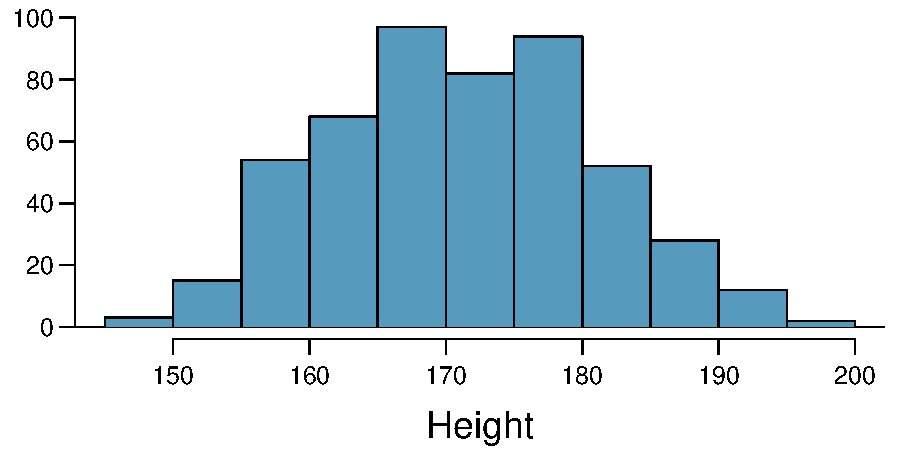
\includegraphics[width=\textwidth]{ch_inference_for_means/figures/eoce/adult_heights/adult_heights_hist.pdf}
\end{center}
\end{minipage}
\begin{minipage}[c]{0.23\textwidth}
\begin{center}
\begin{tabular}{l|r l}
Min     & 147.2 \\
Q1      & 163.8 \\
Median  & 170.3 \\
Mean    & 171.1 \\
SD      &  9.4 \\
Q3      & 177.8 \\
Max     & 198.1 \\
\end{tabular}
\end{center}
\end{minipage}
\begin{parts}
\item What is the point estimate for the average height of active individuals? 
What about the median?
\item What is the point estimate for the standard deviation of the heights of 
active individuals? What about the IQR?
\item Is a person who is 1m 80cm (180 cm) tall considered unusually tall? And is 
a person who is 1m 55cm (155cm) considered unusually short? Explain your 
reasoning.
\item The researchers take another random sample of physically active 
individuals. Would you expect the mean and the standard deviation of this new 
sample to be the ones given above? Explain your reasoning.
\item The sample means obtained are point estimates for the mean height of all 
active individuals, if the sample of individuals is equivalent to a simple 
random sample.
What measure do we use to quantify the variability of such an estimate?
Compute 
this quantity using the data from the original sample under the condition that 
the data are a simple random sample. 
\end{parts}
}{}

% 9

\eoce{\qt{Find the mean\label{find_mean_2_sided}}
You are given the following hypotheses:
\begin{align*}
H_0&: \mu = 60 \\
H_A&: \mu \neq 60
\end{align*}
We know that the sample standard deviation is 8
and the sample size is 20.
For what sample mean would the p-value be equal to 0.05?
Assume that all conditions necessary for inference are satisfied.
}{}

% 10

\eoce{\qt{$t^\star$ vs. $z^\star$\label{critical_t_vs_z}} For a given confidence 
level, $t^{\star}_{df}$ is larger than $z^{\star}$. Explain how $t^{*}_{df}$ 
being slightly larger than $z^{*}$ affects the width of the confidence interval.
}{}

% 11

\eoce{\qt{Play the piano\label{play_piano_2_sided}}
Georgianna claims that in a small city 
renowned for its music school, the average child takes less than 5 years of 
piano lessons. We have a random sample of 20 children from the city, with a 
mean of 4.6 years of piano lessons and a standard deviation of 2.2 years.
\begin{parts}
\item
    Evaluate Georgianna's claim (or that the opposite might be true)
    using a hypothesis test.
\item
    Construct a 95\% confidence interval for the number of years
    students in this city take piano lessons, and interpret it
    in context of the data.
\item
    Do your results from the hypothesis test and the confidence
    interval agree?
    Explain your reasoning.
\end{parts}
}{}

% 12

\eoce{\qt{Auto exhaust and
    lead exposure\label{auto_exhaust_lead_exposure_2_sided}} 
Researchers interested in lead exposure due to car exhaust
sampled the blood of 52 police officers subjected to constant
inhalation of automobile exhaust fumes while working traffic
enforcement in a primarily urban environment.
The blood samples of these officers had an average lead
concentration of 124.32 $\mu$g/l and a SD of 37.74 $\mu$g/l;
a previous study of individuals from a nearby suburb,
with no history of exposure, found an average blood level
concentration 
of 35 $\mu$g/l.\footfullcite{Mortada:2000}
\begin{parts}
\item
    Write down the hypotheses that would be appropriate for
    testing if the police officers appear to have been exposed
    to a different concentration of lead.
\item\label{auto_exhaust_lead_exposure_2_sided_cond}
    Explicitly state and check all conditions necessary for
    inference on these data.
\item
    Regardless of your answers in
    part~(\ref{auto_exhaust_lead_exposure_2_sided_cond}),
    test the hypothesis that the downtown police officers have
    a higher lead exposure than the group in the previous study.
    Interpret your results in context.
\end{parts}
}{}

% 13

\eoce{\qt{Car insurance savings\label{car_insurance_savings}}
A market researcher wants to evaluate car insurance savings
at a competing company.
Based on past studies he is assuming that the standard
deviation of savings is \$100.
He wants to collect data such that he can get a margin of
error of no more than \$10 at a 95\% confidence level.
How large of a sample should he collect?
}{}

% 14

\eoce{\qt{SAT scores\label{sat_scores_CI}}
The standard deviation of SAT scores for students at
a particular Ivy League college is 250 points.
Two statistics students, Raina and Luke, want to estimate
the average SAT score of students at this college as part
of a class project.
They want their margin of error to be no more than 25 points.
\begin{parts}
\item
    Raina wants to use a 90\% confidence interval.
    How large a sample should she collect?
\item
    Luke wants to use a 99\% confidence interval.
    Without calculating the actual sample size, determine
    whether his sample should be larger or smaller
    than Raina's, and explain your reasoning.
\item
    Calculate the minimum required sample size for Luke.
\end{parts}
}{}
}





%__________________
\section{Paired data}
\label{pairedData}

\newcommand{\uclabookN}{68}
\newcommand{\uclabookDF}{67}
\newcommand{\uclabookM}{3.58}
\newcommand{\uclabookSD}{13.42}
\newcommand{\uclabookSE}{1.63}

\index{paired|(}
\index{data!textbooks|(}

\noindent%
In an earlier edition of this textbook,
we found that Amazon prices were, on average,
lower than those of the UCLA Bookstore for UCLA courses
in 2010.
It's been several years, and many stores have adapted
to the online market, so we wondered,
how is the UCLA Bookstore doing today?

We sampled 201 UCLA courses.
Of those, \uclabookN{}
required books could be found on Amazon.
A~portion of the data set from these courses
is shown in Figure~\ref{textbooksDF},
where prices are in US dollars.

\begin{figure}[h]
\centering
\begin{tabular}{r ll ccc}
  \hline
 & subject &
     course\us{}number &
     bookstore &
     amazon &
     price\us{}difference \\ 
  \hline
  1 & American Indian Studies & M10 & 47.97 & 47.45 & 0.52 \\ 
  2 & Anthropology & 2 & 14.26 & 13.55 & 0.71 \\ 
  3 & Arts and Architecture & 10 & 13.50 & 12.53 & 0.97 \\
  $\vdots$ & $\vdots$ & $\vdots$ & $\vdots$ & $\vdots$ & $\vdots$ \\
  %\uclabookDF{} & Korean & 1 & 24.96 & 23.79 & 1.17 \\ 
  \uclabookN{} & Jewish Studies & M10 & 35.96 & 32.40 & 3.56 \\
  \hline
\end{tabular}
\caption{Four cases of the \data{textbooks} data set.%
    \vspace{-3mm}}
\label{textbooksDF}
\end{figure}
% library(openintro); library(xtable); library(dplyr); d <- select(ucla_textbooks_f18, subject, course_num, bookstore_new, amazon_new); d$price_diff <- d$bookstore_new - d$amazon_new; d <- subset(d, !is.na(bookstore_new) & !is.na(amazon_new)); rownames(d) <- NULL; xtable(d[c(1:3, nrow(d) - 1:0),])

\subsection{Paired observations}

Each textbook has two corresponding prices in the data set:
one for the UCLA Bookstore and one for Amazon.
When two sets of observations have this special
correspondence, they are said to be \term{paired}.

\begin{onebox}{Paired data}
  Two sets of observations are \emph{paired} if each
  observation in one set has a special correspondence
  or connection with exactly one observation in the other
  data set.
\end{onebox}

To analyze paired data, it is often useful to look
at the difference in outcomes of each pair of observations.
In the textbook data, we look at the differences
in prices, which is represented as the
\var{price\us{}difference} variable
in the data set.
Here the differences are taken as
\begin{align*}
\text{UCLA Bookstore price} - \text{Amazon price}
\end{align*}
%for each book.
It is important that we always subtract using
a consistent order;
here Amazon prices are always subtracted from UCLA prices.
The first difference shown in Figure~\ref{textbooksDF}
is computed as $47.97 - 47.45 = 0.52$.
Similarly, the second difference is computed as
$14.26 - 13.55 = 0.71$,
 and the third is $13.50 - 12.53 = 0.97$.
A histogram of the differences is shown in
Figure~\ref{diffInTextbookPricesF18}.
Using differences between paired observations
is a common and useful way to analyze paired data.

\begin{figure}[h]
  \centering
  \Figures{0.63}{textbooksF18}{diffInTextbookPricesF18}
  \caption{Histogram of the difference in price for
      each book sampled.}
  \label{diffInTextbookPricesF18}
\end{figure}


\subsection{Inference for paired data}

To analyze a paired data set,
we simply analyze the differences.
We can use the same $t$-distribution techniques
we applied in
Section~\ref{oneSampleMeansWithTDistribution}.

\begin{figure}[h]
\centering
\begin{tabular}{ccccc}
\hline
$n_{_{\text{\emph{diff}}}}$	&\hspace{3mm}& $\bar{x}_{_{\text{\emph{diff}}}}$	&\hspace{3mm}& $s_{_{\text{\emph{diff}}}}$ \vspace{1mm}\\
\uclabookN{}  && \uclabookM{}  && \uclabookSD{} \\
\hline
\end{tabular}
\caption{Summary statistics for the \uclabookN{} price differences.}
\label{textbooksSummaryStats}
\end{figure}

%\Comment{Consider breaking the next example into two pieces.}

\begin{examplewrap}
\begin{nexample}{Set up a hypothesis test
    to determine whether, on average, there is a difference
    between Amazon's price for a book and the UCLA
    bookstore's price.
    Also, check the conditions for whether we can move
    forward with the test using the $t$-distribution.}
  \label{htSetupTextbookPriceDiff}%
  We are considering two scenarios: there is no difference
  or there is some difference in average prices.
  \begin{itemize}
  \setlength{\itemsep}{0mm}
  \item[$H_0$:]
      $\mu_{\text{\emph{diff}}} = 0$.
      There is no difference in the average textbook price.
  \item[$H_A$:]
      $\mu_{\text{\emph{diff}}} \neq 0$.
      There is a difference in average prices.
  \end{itemize}

  Next, we check the independence and normality conditions.
  The observations are based on a simple random sample,
  so independence is reasonable.
  While there are some outliers,
  $n = \uclabookN{}$ and none of the outliers
  are particularly extreme, so the normality
  of $\bar{x}$ is satisfied.
  With these conditions satisfied,
  we can move forward with the $t$-distribution.
\end{nexample}
\end{examplewrap}

\begin{examplewrap}
\begin{nexample}{Complete the hypothesis test started
    in Example~\ref{htSetupTextbookPriceDiff}.}
  \label{SEAndTScoreTextbookPriceDiff}
  To compute the test  compute the standard error associated with
  $\bar{x}_{\text{\emph{diff}}}$ using the standard
  deviation of the differences
  ($s_{_{\text{\emph{diff}}}} = \uclabookSD{}$)
  and the number of differences
  ($n_{_{\text{\emph{diff}}}} = \uclabookN{}$):
  \begin{align*}
  SE_{\bar{x}_{\text{\emph{diff}}}}
    = \frac{s_{\text{\emph{diff}}}}{\sqrt{n_{\text{\emph{diff}}}}}
    = \frac{\uclabookSD{}}{\sqrt{\uclabookN{}}} = \uclabookSE{}
  \end{align*}
  The test statistic is the T-score of
  $\bar{x}_{\text{\emph{diff}}}$
  under the null condition that the actual mean
  difference is~0:
  \begin{align*}
  T
    = \frac{\bar{x}_{\text{\emph{diff}}} - 0}
        {SE_{\bar{x}_{\text{\emph{diff}}}}}
    = \frac{\uclabookM{} - 0}{\uclabookSE{}} = 2.20
  \end{align*}
  To visualize the p-value, the sampling distribution
  of $\bar{x}_{\text{\emph{diff}}}$ is drawn as though
  $H_0$ is true,
  and the p-value is represented by the two shaded tails:
  \begin{center}
  \Figures{0.53}{textbooksF18}{textbooksF18HTTails}
  \end{center}
  The degrees of freedom is
  $df = \uclabookN{} - 1 = \uclabookDF{}$.
  Using statistical software, we find the
  one-tail area of 0.0156.
  Doubling this area gives the p-value: 0.0312.

  Because the p-value is less than 0.05,
  we reject the null hypothesis.
  Amazon prices are, on average, lower than the
  UCLA Bookstore prices for UCLA courses.
\end{nexample}
\end{examplewrap}

\D{\newpage}

\begin{exercisewrap}
\begin{nexercise}
Create a 95\% confidence interval for the average
price difference between books at the UCLA bookstore
and books on Amazon.\footnotemark{}
\end{nexercise}
\end{exercisewrap}
\footnotetext{Conditions
  have already verified and the standard error
  computed in
  Example~\ref{htSetupTextbookPriceDiff}.
  To find the interval,
  identify $t^{\star}_{\uclabookDF{}}$ using statistical software
  or the $t$-table ($t^{\star}_{\uclabookDF{}} = 2.00$),
  and plug it, the point estimate,
  and the standard error into the confidence
  interval formula:
  \begin{align*}
  \text{point estimate} \ \pm\ z^{\star} \times SE
      \quad\to\quad
          \uclabookM{} \ \pm\ 2.00 \times \uclabookSE{}
      \quad\to\quad (0.32, 6.84)
  \end{align*}
  We are 95\% confident that Amazon is, on average,
  between \$0.32 and \$6.84 less expensive
  than the UCLA Bookstore for UCLA course books.}

\begin{exercisewrap}
\begin{nexercise}
We have strong evidence that Amazon is,
on average, less expensive.
How should this conclusion affect UCLA student
buying habits?
Should UCLA students always buy their books
on Amazon?\footnotemark{}
\end{nexercise}
\end{exercisewrap}
\footnotetext{The average price difference
  is only mildly useful for this question.
  Examine the distribution shown in
  Figure~\ref{diffInTextbookPricesF18}.
  There are certainly a handful of cases where
  Amazon prices are far below the UCLA Bookstore's,
  which suggests it is worth checking Amazon
  (and probably other online sites) before purchasing.
  However, in many cases the Amazon price is
  above what the UCLA Bookstore charges,
  and most of the time the price isn't that different.
  Ultimately, if getting a book immediately from
  the bookstore is notably more convenient,
  e.g. to get started on reading or homework,
  it's likely a good idea to go with the UCLA
  Bookstore unless the price difference on a
  specific book happens to be quite large.

  For reference, this is a very different result
  from what we (the authors) had seen in a similar
  data set from 2010.
  At that time, Amazon prices were almost uniformly
  lower than those of the UCLA Bookstore's and by
  a large margin, making the case to use Amazon over
  the UCLA Bookstore quite compelling at that time.
  Now we frequently check multiple websites
  to find the best price.}

\index{data!textbooks|)}
\index{paired|)}

{


%_______________
\newpage\subsection*{Exercises} % Paired data

% 1

\eoce{\qt{Air quality\label{air_quality}} Air quality measurements were collected in 
a random sample of 25 country capitals in 2013, and then again in the same 
cities in 2014. We would like to use these data to compare average air quality 
between the two years.
\begin{parts}
\item Should we use a one-sided or a two-sided test? Explain your reasoning.
\item Should we use a paired or non-paired test? Explain your reasoning.
\item Should we use a $t$-test or a $z$-test? Explain your reasoning.
\end{parts}
}{}

% 2

\eoce{\qt{True / False: paired\label{tf_paired}} Determine if the following 
statements are true or false. If false, explain.
\begin{parts}
\item In a paired analysis we first take the difference of each pair of observations, 
and then we do inference on these differences.
\item Two data sets of different sizes cannot be analyzed as paired data.
\item Consider two sets of data that are paired with each other.
Each observation in one data set has a natural correspondence with 
exactly one observation from the other data set.
\item Consider two sets of data that are paired with each other.
Each observation in one data set is subtracted from the average of the 
other data set's observations.
\end{parts}
}{}

% 3

\eoce{\qt{Paired or not? Part I\label{paired_or_not_1}} In each of the following 
scenarios, determine if the data are paired.
\begin{parts}
\item Compare pre- (beginning of semester) and post-test (end of semester) 
scores of students.
\item Assess gender-related salary gap by comparing salaries of randomly 
sampled men and women.
\item Compare artery thicknesses at the beginning of a study and after 2 years 
of taking Vitamin E for the same group of patients.
\item Assess effectiveness of a diet regimen by comparing the before and after 
weights of subjects.
\end{parts}
}{}

% 4

\eoce{\qt{Paired or not? Part II\label{paired_or_not_2}} In each of the following 
scenarios, determine if the data are paired.
\begin{parts}
\item We would like to know if Intel's stock and Southwest Airlines' stock have 
similar rates of return. To find out, we take a random sample of 50 days, and 
record Intel's and Southwest's stock on those same days.
\item We randomly sample 50 items from Target stores and note the price for 
each. Then we visit Walmart and collect the price for each of those same 50 
items.
\item A school board would like to determine whether there is a difference in 
average SAT scores for students at one high school versus another high school 
in the district. To check, they take a simple random sample of 100 students 
from each high school.
\end{parts}
}{}

% 5

\eoce{\qt{Global warming, Part I\label{global_warming_v2_1}}
\textbf{\color{red}ADD SOLUTION}
Is there strong evidence of global warming?
Let's consider a small scale example.
We sampled 197 locations from the NOAA's historical data
(NOAA stands for National Oceanic and Atmospheric Administration),
where the data was available for both 1948 and 2018.
We want to know: were there more days with temperatures
exceeding 90\textdegree{}F in 2018 than
in~1948.\footfullcite{webpage:noaa_1948_2018}
The difference in number of days exceeding 90\textdegree{}F
(number of days in 2018 - number of days in 1948) was calculated
for each of the 197 locations.
The average of these differences was 2.9 days with 
a standard deviation of 17.2 days.
We are interested in determining whether these data provide
strong evidence that there were more days in 2018 that
exceeded 90\textdegree{}F from NOAA's weather stations.
\begin{parts}
\item
    Is there a relationship between the observations collected
    in 1948 and 2018?
    Or are the observations in the two groups independent?
    Explain.
\item
    Write hypotheses for this research in symbols and in words.
\item
    Check the conditions required to complete this test.
\item
    Calculate the test statistic and find the p-value.
\item
    What do you conclude?
    Interpret your conclusion in context.
\item
    What type of error might we have made?
    Explain in context what the error means.
\item
    Based on the results of this hypothesis test,
    would you expect a confidence interval for the
    average difference between the number of days
    exceeding 90\textdegree{}F from 1948 and 2018
    to include 0?
    Explain your reasoning.
\end{parts}
% library(openintro); d <- climate70$dx90_2018 - climate70$dx90_1948; mean(d); sd(d); length(d); t.test(d)
}{}

% 6

\eoce{\qt{High School and Beyond, Part I\label{hs_beyond_1}} The National Center of 
Education Statistics conducted a survey of high school seniors, collecting test 
data on reading, writing, and several other subjects. Here we examine a simple 
random sample of 200 students from this survey. Side-by-side box plots of 
reading and writing scores as well as a histogram of the differences in scores 
are shown below.
\begin{center}
\includegraphics[width=0.44\textwidth]{ch_inference_for_means/figures/eoce/hs_beyond_1/hs_beyond_read_write_box.pdf}
\includegraphics[width=0.54\textwidth]{ch_inference_for_means/figures/eoce/hs_beyond_1/hs_beyond_diff_hist.pdf}
\end{center}
\begin{parts}
\item Is there a clear difference in the average reading and writing scores?
\item Are the reading and writing scores of each student independent of each 
other?
\item Create hypotheses appropriate for the following research question: is 
there an evident difference in the average scores of students in the reading 
and writing exam?
% is there evidence that students on average perform differently on the reading and writing exam?
\item Check the conditions required to complete this test.
\item The average observed difference in scores is 
$\bar{x}_{read-write} = -0.545$, and the standard deviation of the differences 
is 8.887 points. Do these data provide convincing evidence of a difference 
between the average scores on the two exams?
\item What type of error might we have made? Explain what the error means in 
the context of the application.
\item Based on the results of this hypothesis test, would you expect a 
confidence interval for the average difference between the reading and writing 
scores to include 0? Explain your reasoning.
\end{parts}
}{}

% 7

\eoce{\qt{Global warming, Part II\label{global_warming_v2_2}}
\textbf{\color{red}ADD SOLUTION.}
We considered the change in the number of days exceeding
90\textdegree{}F from 1948 and 2018 at 197 randomly sampled
locations from the NOAA database in
Exercise~\ref{global_warming_v2_1}.
The mean and standard deviation of the reported differences
are 2.9 days and 17.2 days.
\begin{parts}
\item
    Calculate a 90\% confidence interval for the average
    difference between number of days exceeding 90\textdegree{}F
    between 1948 and 2018.
\item
    Interpret this interval in context.
\item
    Does the confidence interval provide convincing evidence
    that the temperature was higher in 2008 than in 1968 in
    the continental US?
    Explain.
\end{parts}
}{}

% 8

\eoce{\qt{High school and beyond, Part II\label{hs_beyond_2}} We considered the 
differences between the reading and writing scores of a random sample of 200 
students who took the High School and Beyond Survey in Exercise~\ref{hs_beyond_1}. The 
mean and standard deviation of the differences are 
$\bar{x}_{read-write} = -0.545$ and 8.887 points.
\begin{parts}
\item Calculate a 95\% confidence interval for the average difference between 
the reading and writing scores of all students.
\item Interpret this interval in context.
\item Does the confidence interval provide convincing evidence that there is a 
real difference in the average scores? Explain.
\end{parts}
}{}
}






%__________________
\section{Difference of two means}
\label{differenceOfTwoMeans}

\noindent%
In this section we consider a difference in
two population means, $\mu_1 - \mu_2$, under the condition
that the data are not paired.
Just as with a single sample, we identify conditions to ensure
we can use the $t$-distribution with a point estimate
of the difference, $\bar{x}_1 - \bar{x}_2$,
and a new standard error formula.
Other than these two differences, the details are almost
identical to the one-mean procedures.

We apply these methods in three contexts: determining whether
stem cells can improve heart function,
exploring the relationship between pregnant womens' smoking
habits and birth weights of newborns,
and exploring whether there is statistically significant
evidence that one variation of an exam is harder than
another variation.
This section is motivated by questions like
``Is there convincing evidence that newborns from mothers
who smoke have a different average birth weight than newborns
from mothers who don't smoke?''


\subsection{Confidence interval for a difference of means}

\index{data!stem cells, heart function|(}
\index{point estimate!difference of means|(}

Does treatment using embryonic stem cells (ESCs)
help improve heart function following a heart attack?
Figure~\ref{statsSheepEscStudy} contains summary statistics
for an experiment to test ESCs in sheep that had a heart attack.
Each of these sheep was randomly assigned to the ESC
or control group, and the change in their hearts' pumping
capacity was measured in the study.
Figure~\ref{stemCellTherapyForHearts} provides
histograms of the two data sets.
A~positive value corresponds to increased pumping capacity,
which generally suggests a stronger recovery.
Our goal will be to identify a 95\% confidence interval
for the effect of ESCs on the change in heart pumping
capacity relative to the control group.

\begin{figure}[h]
\centering
\begin{tabular}{l rrrrr}
\hline
\hspace{10mm}	& $n$	& $\bar{x}$	& $s$  \\
\hline
ESCs     & 9  & 3.50   & 5.17  \\
control  & 9  & -4.33  & 2.76  \\
\hline
\end{tabular}
\caption{Summary statistics of the embryonic stem cell study.}
\label{statsSheepEscStudy}
\end{figure}

The point estimate of the difference in the heart pumping variable
is straightforward to find: it is the difference in the sample means.
\begin{align*}
\bar{x}_{esc} - \bar{x}_{control}\ 
  =\ 3.50 - (-4.33)\ 
  =\ 7.83
\end{align*}
For the question of whether we can model this difference
using a $t$-distribution, we'll need to check new conditions.
Like the 2-proportion cases, we will require a more
robust version of independence so we are confident
the two groups are also independent.
Secondly, we also check for normality in each
group separately, which in practice is a check
for outliers.

\index{point estimate!difference of means|)}

%\begin{examplewrap}
%\begin{nexample}{Set up hypotheses that will be used to test whether there is convincing evidence that ESCs actually increase the amount of blood the heart pumps. Also, check conditions for using the $t$-distribution for inference with the point estimate $\bar{x}_1 - \bar{x}_2$. To assist in this assessment, the data are presented in Figure~\ref{stemCellTherapyForHearts}.}\label{exampleToEvaluteWhetherESCsAreHelpfulInImprovingHeartFunctionInSheep}
%We first setup the hypotheses:
%\begin{itemize}
%\setlength{\itemsep}{0mm}
%\item[$H_0$:] The stem cells do not improve heart pumping function. $\mu_{esc} - \mu_{control} = 0$.
%\item[$H_A$:] The stem cells do improve heart pumping function. $\mu_{esc} - \mu_{control} > 0$.
%\end{itemize}
%\end{nexample}
%\end{examplewrap}

\begin{onebox}{Using the
    $\pmb{\MakeLowercase{t}}$-distribution
    for a difference in means}
  \label{ConditionsForTwoSampleTDist}%
  The $t$-distribution can be used for inference when working
  with the standardized difference of two means if
  \begin{itemize}
  \setlength{\itemsep}{0mm}
  \item \emph{Independence, extended.}
    The data are independent within and between
    the two groups, e.g. the data come from
    independent random samples or from a
    randomized experiment.
  \item \emph{Normality.}
    We check the outliers rules of thumb for
    each group separately.
  \end{itemize}
  The standard error may be computed as
  \begin{align*}
  SE%_{\bar{x}_{1} - \bar{x}_{2}}
    = \sqrt{\frac{\sigma_1^2}{n_1} + \frac{\sigma_2^2}{n_2}}
    %\approx \sqrt{\frac{s_1^2}{n_1} + \frac{s_2^2}{n_2}}
  \index{standard error (SE)!difference in means}
  \end{align*}
  The official formula for the degrees of freedom is quite
  complex %\footnotemark{}
  and is generally computed using software,
  so instead you may use the smaller of
  $n_1 - 1$ and $n_2 - 1$ for the degrees of freedom
  if software isn't readily available.
\end{onebox}
%\footnotetext{$df = 
%    \left.
%    \left[\frac{s_1^2}{n_1} + \frac{s_2^2}{n_2}\right]^2
%    \middle/
%    \left[\frac{(s_1^2 / n_1)^2}{n_1 - 1} +
%        \frac{(s_2^2 / n_2)^2}{n_2 - 1}\right]
%    \right.$}


\D{\newpage}

\begin{examplewrap}
\begin{nexample}{Can the $t$-distribution be used to make
    inference using the point estimate,
    $\bar{x}_{esc} - \bar{x}_{control} = 7.83$?}
  First, we check for independence.
  Because the sheep were randomized into
  the groups, independence within
  and between groups is satisfied.

  Figure~\ref{stemCellTherapyForHearts}
  does not reveal any clear outliers
  in either group.
  (The ESC group does look a bit more variability,
  but this is not the same as having clear outliers.)

  With both conditions met, we can use the
  $t$-distribution to model the difference of sample means.
\end{nexample}
\end{examplewrap}

\begin{figure}[h]
  \centering
  \Figure{0.63}{stemCellTherapyForHearts}
  \caption{Histograms for both the embryonic stem cell
      and control group.}
  \label{stemCellTherapyForHearts}
\end{figure}

%\begin{onebox}{Conditions for applying the $t$-distribution to $\bar{x}_1 - \bar{x}_2$}
%If the sample means, $\bar{x}_1$ and $\bar{x}_2$, each meet the criteria for using the $t$-distribution and the observations in the two samples are independent, then we can analyze the difference in sample means using the $t$-distribution.
%\end{onebox}

%In addition to new conditions, we also will need an updated
%formula for the standard error for the difference of two means.
%
%\begin{onebox}{Distribution of a difference of sample means}
%  The sample difference of two means, $\bar{x}_1 - \bar{x}_2$,
%  can be modeled using the $t$-distribution and the standard error
%  \begin{align*}
%  SE%_{\bar{x}_{1} - \bar{x}_{2}}
%    = \sqrt{\frac{\sigma_1^2}{n_1} + \frac{\sigma_2^2}{n_2}}
%    %\approx \sqrt{\frac{s_1^2}{n_1} + \frac{s_2^2}{n_2}}
%  \end{align*}
%  when each sample mean can itself be modeled using
%  a $t$-distribution and the samples are independent.
%  The official formula for the degrees of freedom is quite
%  complex %\footnotemark{}
%  and is generally computed using software,
%  so instead you may use the smaller of
%  $n_1 - 1$ and $n_2 - 1$ for the degrees of freedom
%  if software isn't readily available.
%\end{onebox}
%%\footnotetext{$df = 
%%    \left.
%%    \left[\frac{s_1^2}{n_1} + \frac{s_2^2}{n_2}\right]^2
%%    \middle/
%%    \left[\frac{(s_1^2 / n_1)^2}{n_1 - 1} +
%%        \frac{(s_2^2 / n_2)^2}{n_2 - 1}\right]
%%    \right.$}

%We can quantify the variability in the point estimate,
%$\bar{x}_{esc} - \bar{x}_{\text{control}}$,
%using the following formula for its standard error:
%\index{standard error (SE)!difference in means}
%\begin{align*}
%SE%_{\bar{x}_{esc} - \bar{x}_{control}}
%  = \sqrt{\frac{\sigma_{esc}^2}{n_{esc}}
%      + \frac{\sigma_{control}^2}{n_{control}}}
%\end{align*}
As with the one-sample case, we always compute the
standard error using sample standard deviations rather
than population standard deviations:
\begin{align*}
SE%_{\bar{x}_{esc} - \bar{x}_{control}}
	%= \sqrt{\frac{\sigma_{esc}^2}{n_{esc}} + \frac{\sigma_{control}^2}{n_{control}}} %\\
	= \sqrt{\frac{s_{esc}^2}{n_{esc}} + \frac{s_{control}^2}{n_{control}}}
	= \sqrt{\frac{5.17^2}{9} + \frac{2.76^2}{9}} = 1.95
\end{align*}
Generally, we use statistical software to find the appropriate
degrees of freedom, or if software isn't available,
we can use the smaller
of $n_1 - 1$ and $n_2 - 1$ for the degrees of freedom,
e.g. if using a $t$-table to find tail areas.
For transparency in the Examples and Guided Practice,
we'll use the latter approach for finding $df$;
in the case of the ESC example, this means we'll use $df = 8$.

\begin{examplewrap}
\begin{nexample}{Calculate a 95\% confidence interval for the
    effect of ESCs on the change in heart pumping capacity of
    sheep after they've suffered a heart attack.}
  We will use the sample difference and the standard error that 
  we computed earlier calculations:
  \begin{align*}
  \bar{x}_{esc} - \bar{x}_{control} = 7.83
  && SE = \sqrt{\frac{5.17^2}{9} + \frac{2.76^2}{9}} = 1.95
  \end{align*}
  Using $df = 8$, we can identify the
  critical value of $t^{\star}_{8} = 2.31$
  for a 95\% confidence interval.
  Finally, we can enter the values into the confidence
  interval formula:
  \begin{align*}
  \text{point estimate} \ \pm\ t^{\star} \times SE
    \quad\rightarrow\quad 7.83 \ \pm\ 2.31\times 1.95
    \quad\rightarrow\quad (3.32, 12.34)
  \end{align*}
  We are 95\% confident that embryonic stem cells improve
  the heart's pumping function in sheep that have suffered
  a heart attack by 3.32\% to 12.34\%.
  
%  Had we used software to get a more precise degrees
%  of freedom ($df = 12.225$), the confidence interval
%  would have been slightly slimmer.
\end{nexample}
\end{examplewrap}

\index{data!stem cells, heart function|)}

\noindent%
As with past statistical inference applications,
there is a well-trodden procedure.
\begin{description}
\setlength{\itemsep}{0mm}
\item[Prepare.]
    Retrieve critical contextual information,
    and if appropriate, set up hypotheses.
\item[Check.]
    Ensure the required conditions are reasonably
    satisfied.
\item[Calculate.]
    Find the standard error, and then construct
    a confidence interval, or if conducting
    a hypothesis test, find a test statistic
    and p-value.
\item[Conclude.]
    Interpret the results in the context of the
    application.
\end{description}
The details change a little from one setting to the next,
but this general approach remain the same.


%\D{\newpage}

\subsection{Hypothesis tests for the difference of two means}

\index{data!baby\_smoke|(}

A data set called \data{ncbirths} represents a random sample of 150 cases of mothers and their newborns in North Carolina over a year. Four cases from this data set are represented in Figure~\ref{babySmokeDF}. We are particularly interested in two variables: \var{weight} and \var{smoke}. The \var{weight} variable represents the weights of the newborns and the \var{smoke} variable describes which mothers smoked during pregnancy. We would like to know, is there convincing evidence that newborns from mothers who smoke have a different average birth weight than newborns from mothers who don't smoke? We will use the North Carolina sample to try to answer this question. The smoking group includes 50 cases and the nonsmoking group contains 100 cases.
%Figure~\ref{babySmokePlotOfTwoGroupsToExamineSkew}.

\begin{figure}[h]
\centering
\begin{tabular}{rrrrrll}
  \hline
 & fage & mage & weeks & weight & sex & smoke \\ 
  \hline
1 & NA & 13 &  37 & 5.00 & female & nonsmoker \\ 
  2 & NA & 14 &  36 & 5.88 & female & nonsmoker \\ 
  3 & 19 & 15 &  41 & 8.13 & male & smoker \\ 
  $\vdots$ &   $\vdots$ &   $\vdots$ &   $\vdots$ &   $\vdots$ &   $\vdots$ \\
  150 & 45 & 50 &  36 & 9.25 & female & nonsmoker \\ 
   \hline
\end{tabular}
\caption{Four cases from the \data{ncbirths} data set. The value ``NA'', shown for the first two entries of the first variable, indicates that piece of data is missing.}
\label{babySmokeDF}
\end{figure}

\begin{examplewrap}
\begin{nexample}{Set up appropriate hypotheses to evaluate
    whether there is a relationship between a mother smoking
    and average birth weight.}
  \label{babySmokeHTForWeight}%
  The null hypothesis represents the case of no difference
  between the groups.
  \begin{itemize}
  \setlength{\itemsep}{0mm}
  \item[$H_0$:]
      There is no difference in average birth weight for
      newborns from mothers who did and did not smoke.
      In statistical notation: $\mu_{n} - \mu_{s} = 0$,
      where $\mu_{n}$ represents non-smoking mothers and
      $\mu_s$ represents mothers who smoked.
  \item[$H_A$:]
      There is some difference in average newborn weights
      from mothers who did and did not smoke
      ($\mu_{n} - \mu_{s} \neq 0$).
  \end{itemize}
\end{nexample}
\end{examplewrap}

We check the two conditions necessary to model the difference
in sample means using the $t$-distribution.
\begin{itemize}
\item
    Because the data come from a simple random sample,
    the observations are independent,
    both within and between samples.
\item
    With both data sets over 30 observations,
    we inspect the data in
    Figure~\ref{babySmokePlotOfTwoGroupsToExamineSkew}
    for any particularly extreme outliers
    and find none.
\end{itemize}
Since both conditions are satisfied, the difference
in sample means may be modeled using a $t$-distribution.

\begin{figure}[hhh]
  \centering
  \Figure{}{babySmokePlotOfTwoGroupsToExamineSkew}
  \caption{The top panel represents birth weights for infants
      whose mothers smoked.
      The bottom panel represents the birth weights for
      infants whose mothers who did not smoke.}
  \label{babySmokePlotOfTwoGroupsToExamineSkew}
\end{figure}

%Summary statistics are shown for each sample in Figure~\ref{SumStatsBirthWeightNewbornsSmoke}.

%\D{\newpage}

\begin{exercisewrap}
\begin{nexercise}
\label{babySmokeCalcForWeight}
The summary statistics in
Figure~\ref{SumStatsBirthWeightNewbornsSmoke} may be useful
for this Guided Practice.\footnotemark{}
\begin{enumerate}[(a)]
\setlength{\itemsep}{0mm}
\item
    What is the point estimate of the population difference,
    $\mu_{n} - \mu_{s}$?
\item
    Compute the standard error of the point estimate from
    part~(a).
\end{enumerate}
\end{nexercise}
\end{exercisewrap}
\footnotetext{(a)~The difference in sample means is an
  appropriate point estimate: $\bar{x}_{n} - \bar{x}_{s} = 0.40$.
  (b)~The standard error of the estimate can be
  calculated using the standard error formula:
  \begin{align*}
  SE
    = \sqrt{\frac{\sigma_n^2}{n_n} + \frac{\sigma_s^2}{n_s}}
      \approx \sqrt{\frac{s_n^2}{n_n} + \frac{s_s^2}{n_s}}
    = \sqrt{\frac{1.60^2}{100} + \frac{1.43^2}{50}}
    = 0.26
  \end{align*}}

\begin{figure}[hhh]
\centering
\begin{tabular}{lrr}
\hline
& \resp{smoker} & \resp{nonsmoker} \\
\hline
mean & 6.78 & 7.18 \\
st. dev. & 1.43 & 1.60 \\
samp. size & 50 & 100 \\
\hline
\end{tabular}
\caption{Summary statistics for the \data{ncbirths} data set.}
\label{SumStatsBirthWeightNewbornsSmoke}
\end{figure}

\D{\newpage}

\begin{examplewrap}
\begin{nexample}{Complete the
    hypothesis test started in
    Example~\ref{babySmokeHTForWeight}
    and Guided Practice~\ref{babySmokeCalcForWeight}.
    Use a significance level of $\alpha=0.05$.
    For reference, $\bar{x}_{n} - \bar{x}_{s} = 0.40$,
    $SE = 0.26$, and the sample sizes were $n_n = 100$
    and $n_s = 50$.}
  \label{babySmokeHTForWeightComputePValueAndEvalHT}%
  We can find the test statistic for this test
  using the values from
  Guided Practice~\ref{babySmokeCalcForWeight}:
  \begin{align*}
  T = \frac{\ 0.40 - 0\ }{0.26} = 1.54
  \end{align*}
  The p-value is represented by the two shaded tails
  in the following plot:
  \begin{center}
    \Figure{0.5}{distOfDiffOfSampleMeansForBWOfBabySmokeData}
  \end{center}
  We find the single tail area using software
  (or the $t$-table in Appendix~\ref{tDistributionTable}).
  We'll use the
  smaller of $n_n - 1 = 99$ and $n_s - 1 = 49$ as the
  degrees of freedom: $df = 49$.
  The one tail area is 0.065;
  doubling this value gives the two-tail area and p-value,
  0.135.

  The p-value is larger than the significance value, 0.05,
  so we do not reject the null hypothesis.
  There is insufficient evidence to say there is a difference
  in average birth weight of newborns from North Carolina mothers
  who did smoke during pregnancy and newborns from North Carolina
  mothers who did not smoke during pregnancy.
\end{nexample}
\end{examplewrap}

%\D{\newpage}

\begin{exercisewrap}
\begin{nexercise}
We've seen much research suggesting smoking is harmful
during pregnancy, so how could we fail to reject the null
hypothesis in
Example~\ref{babySmokeHTForWeightComputePValueAndEvalHT}?
\footnotemark{}
\end{nexercise}
\end{exercisewrap}
\footnotetext{It is possible that there is a difference
  but we did not detect it.
  If there is a difference, we made a Type~2 Error.}

\begin{exercisewrap}
\begin{nexercise}
\label{babySmokeHTIDingHowToDetectDifferences}%
If we made a Type~2 Error and there is a difference,
what could we have done differently in data collection
to be more likely to detect the difference?\footnotemark{}
\end{nexercise}
\end{exercisewrap}
\footnotetext{We could have collected more data.
  If the sample sizes are larger, we tend to have
  a better shot at finding a difference if one exists.
  In fact, this is exactly what we would find if we
  examined a larger data set!}

Public service announcement: while we have used this relatively
small data set as an example, larger data sets show that women
who smoke tend to have smaller newborns.
In~fact, some in the tobacco industry actually had the audacity
to tout that as a \emph{benefit} of~smoking:
\begin{quotation}
  \noindent%
  \emph{It's true.
  The babies born from women who smoke are smaller,
  but they're just as healthy as the babies born from
  women who do not smoke.
  And some women would prefer having smaller babies.} \\[2mm]
  \indent\indent\indent\indent\indent\indent%
    - Joseph Cullman, Philip Morris' Chairman of the Board \\
  \indent\indent\indent\indent\indent\indent%
  {\color{white}...}on CBS' \emph{Face the Nation}, Jan 3,~1971
\end{quotation}
Fact check: the babies from women who smoke are not actually
as healthy as the babies from women who do not
smoke.\footnote{You can watch an episode of John Oliver
  on \emph{Last Week Tonight} to explore the present day
  offenses of the tobacco industry.
  Please be aware that there is some adult language:
  \oiRedirect{textbook-johnoliver_tobacco}{youtu.be/6UsHHOCH4q8}.}
% Resource on this topic:
% http://archive.tobacco.org/Documents/documentquotes.html

\index{data!baby\_smoke|)}


\D{\newpage}

\subsection{Case study: two versions of a course exam}

\index{data!two exam comparison|(}

An instructor decided to run two slight variations of the same exam. Prior to passing out the exams, she shuffled the exams together to ensure each student received a random version. Summary statistics for how students performed on these two exams are shown in Figure~\ref{summaryStatsForTwoVersionsOfExams}. Anticipating complaints from students who took Version~B, she would like to evaluate whether the difference observed in the groups is so large that it provides convincing evidence that Version~B was more difficult (on average) than Version~A.

\begin{figure}[hht]
\centering
\begin{tabular}{l rrrrr}
\hline
Version\hspace{2mm}	& $n$	& $\bar{x}$	& $s$	& min	& max  \\
\hline
A		& 30		& 79.4		& 14 	& 45		& 100 \\
B		& 27		& 74.1		& 20		& 32		& 100 \\
\hline
\end{tabular}
\caption{Summary statistics of scores for each exam version.}
\label{summaryStatsForTwoVersionsOfExams}
\end{figure}

\begin{exercisewrap}
\begin{nexercise}
\label{htSetupForEvaluatingTwoExamVersions}%
Construct hypotheses to evaluate whether the observed
difference in sample means, $\bar{x}_A - \bar{x}_B=5.3$,
is due to chance. We will later evaluate these hypotheses
using $\alpha = 0.01$.\footnotemark{}
\end{nexercise}
\end{exercisewrap}
\footnotetext{$H_0$: the exams are equally difficult, on average. $\mu_A - \mu_B = 0$. $H_A$: one exam was more difficult than the other, on average. $\mu_A - \mu_B \neq 0$.}

%\D{\newpage}

\begin{exercisewrap}
\begin{nexercise} \label{conditionsForTDistForEvaluatingTwoExamVersions}%
To evaluate the hypotheses in Guided Practice~\ref{htSetupForEvaluatingTwoExamVersions} using the $t$-distribution, we must first verify conditions.\footnotemark{}
\begin{enumerate}[(a)]
\setlength{\itemsep}{0mm}
\item
    Does it seem reasonable that the scores are independent?
\item
    Any concerns about outliers?
\end{enumerate}
\end{nexercise}
\end{exercisewrap}
\footnotetext{(a)~Since the exams were shuffled,
  the ``treatment'' in this case was randomly assigned,
  so independence within and between groups is satisfied.
  (b)~The summary statistics suggest the data are roughly
  symmetric about the mean, and the min/max values don't
  suggest any outliers of concern.}

After verifying the conditions for each sample and confirming the samples are independent of each other, we are ready to conduct the test using the $t$-distribution. In this case, we are estimating the true difference in average test scores using the sample data, so the point estimate is $\bar{x}_A - \bar{x}_B = 5.3$. The standard error of the estimate can be calculated~as
\begin{align*}
SE
  = \sqrt{\frac{s_A^2}{n_A} + \frac{s_B^2}{n_B}}
  = \sqrt{\frac{14^2}{30} + \frac{20^2}{27}}
  = 4.62
\end{align*}
Finally, we construct the test statistic:
\begin{align*}
T
  = \frac{\text{point estimate} - \text{null value}}{SE}
  = \frac{(79.4-74.1) - 0}{4.62}
  = 1.15
\end{align*}
If we have a computer handy, we can identify the degrees
of freedom as 45.97.
Otherwise we use the smaller of $n_1-1$ and $n_2-1$: $df=26$.

\D{\newpage}

\begin{figure}[h]
  \centering
  \Figure{0.63}{pValueOfTwoTailAreaOfExamVersionsWhereDFIs26}
  \caption{The $t$-distribution with 26 degrees of freedom
      and the p-value from exam example represented
      as the shaded areas.}
  \label{pValueOfTwoTailAreaOfExamVersionsWhereDFIs26}
\end{figure}

\begin{examplewrap}
\begin{nexample}{Identify the p-value depicted in
    Figure~\ref{pValueOfTwoTailAreaOfExamVersionsWhereDFIs26}
    using $df = 26$, and provide a conclusion in the
    context of the case study.}
  Using software, we can find the one-tail area (0.13)
  and then double this value to get the two-tail area,
  which is the p-value: 0.26.
  (Alternatively, we could use the $t$-table in
  Appendix~\ref{tDistributionTable}.)

  In Guided
  Practice~\ref{htSetupForEvaluatingTwoExamVersions},
  we specified that we would use $\alpha = 0.01$.
  Since the p-value is larger than $\alpha$,
  we do not reject the null hypothesis.
  That is, the data do not convincingly show that one exam
  version is more difficult than the other, and the teacher
  should not be convinced that she should add points to the
  Version~B exam scores.
\end{nexample}
\end{examplewrap}

\index{data!two exam comparison|)}

%\subsection{Summary for inference using the $t$-distribution}
%
%\Comment{This subsection should be heavily updated.}
%
%%When considering the difference of two means, there are two common cases: the two samples are paired or they are independent. (There are instances where the data are neither paired nor independent, e.g. see blocking in Section~\ref{experimentalDesignPrinciples}.) The paired case was treated in Section~\ref{pairedData}, where the one-sample methods were applied to the differences from the paired observations. We examined the second and more complex scenario in this section.
%
%\textbf{Hypothesis tests.} When applying the $t$-distribution for a hypothesis test, we proceed as follows:
%\begin{itemize}
%\setlength{\itemsep}{0mm}
%\item Write appropriate hypotheses.
%\item Verify conditions for using the $t$-distribution.
%\begin{itemize}
%\item One-sample or differences from paired data: the observations (or differences) must be independent and nearly normal. For larger sample sizes, we can relax the nearly normal requirement, e.g. slight skew is okay for sample sizes of 15, moderate skew for sample sizes of 30, and strong skew for sample sizes of 60.
%\item For a difference of means when the data are not paired: each sample mean must separately satisfy the one-sample conditions for the $t$-distribution, and the data in the groups must also be independent.
%\end{itemize}
%\item Compute the point estimate of interest, the standard error, and the degrees of freedom. For $df$, use $n-1$ for one sample, and for two samples use either statistical software or the smaller of $n_1 - 1$ and $n_2 - 1$.
%\item Compute the T-score and p-value.
%\item Make a conclusion based on the p-value, and write a conclusion in context and in plain language so anyone can understand the result.
%\end{itemize}
%\noindent\textbf{Confidence intervals.} Similarly, the following is how we generally computed a confidence interval using a $t$-distribution:
%\begin{itemize}
%\item Verify conditions for using the $t$-distribution. (See above.)
%\item Compute the point estimate of interest, the standard error, the degrees of freedom, and $t^{\star}_{df}$.
%\item Calculate the confidence interval using the general formula, point estimate $\pm\ t_{df}^{\star} SE$.
%\item Put the conclusions in context and in plain language so even non-data scientists can understand the results.
%\end{itemize}
%
%\CalculatorVideos{confidence intervals and hypothesis tests for a difference of means}


%\subsection{Examining the standard error formula (special topic)}
%
%The formula for the standard error of the difference in two means is similar to the formula for other standard errors. Recall that the standard error of a single mean, $\bar{x}_1$, can be approximated by
%\begin{align*}
%SE_{\bar{x}_1} = \frac{s_1}{\ \sqrt{n_1}\ }
%\end{align*}
%where $s_1$ and $n_1$ represent the sample standard deviation and sample size.
%
%The standard error of the difference of two sample means can be constructed from the standard errors of the separate sample means:
%\begin{align*}
%SE_{\bar{x}_{1} - \bar{x}_{2}}
%	= \sqrt{SE_{\bar{x}_1}^2 + SE_{\bar{x}_2}^2}
%	= \sqrt{\frac{s_1^2}{{n_1}} + \frac{s_2^2}{{n_2}}}
%\end{align*}
%This special relationship follows from probability theory.
%
%\begin{exercisewrap}
%\begin{nexercise}
%\label{derivingSEForDiffOfTwoMeansExercise}%
%Prerequisite: Section~\ref{randomVariablesSection}.
%We can rewrite the equation above in a different way:
%\begin{align*}
%SE_{\bar{x}_{1} - \bar{x}_{2}}^2
%  = SE_{\bar{x}_1}^2 + SE_{\bar{x}_2}^2
%\end{align*}
%Explain where this formula comes from using the ideas of probability theory.\footnotemark{}
%\end{nexercise}
%\end{exercisewrap}
%\footnotetext{The standard error squared represents the variance of the estimate. If $X$ and $Y$ are two random variables with variances $\sigma_x^2$ and $\sigma_y^2$, then the variance of $X-Y$ is $\sigma_x^2 + \sigma_y^2$. Likewise, the variance corresponding to $\bar{x}_1 - \bar{x}_2$ is $\sigma_{\bar{x}_1}^2 + \sigma_{\bar{x}_2}^2$. Because $\sigma_{\bar{x}_1}^2$ and $\sigma_{\bar{x}_2}^2$ are just another way of writing $SE_{\bar{x}_1}^2$ and  $SE_{\bar{x}_2}^2$, the variance associated with $\bar{x}_1 - \bar{x}_2$ may be written as $SE_{\bar{x}_1}^2 + SE_{\bar{x}_2}^2$.}


%\D{\newpage}

\subsection{Pooled standard deviation estimate (special topic)}
\label{pooledStandardDeviations}

Occasionally, two populations will have standard deviations
that are so similar that they can be treated as identical.
For example, historical data or a well-understood biological
mechanism may justify this strong assumption.
In such cases, we can make the $t$-distribution approach
slightly more precise by using a pooled standard deviation.

The \term{pooled standard deviation} of two groups is a way
to use data from both samples to better estimate the standard
deviation and standard error.
If $s_1^{}$ and $s_2^{}$ are the standard deviations
of groups~1 and~2 and there are very good reasons to believe
that the population standard deviations are equal,
then we can obtain an improved estimate of the group variances
by pooling their data:
\begin{align*}
s_{pooled}^2 = \frac{s_1^2\times (n_1-1) + s_2^2\times (n_2-1)}{n_1 + n_2 - 2}
\end{align*}
where $n_1$ and $n_2$ are the sample sizes, as before.
To use this new statistic, we substitute $s_{pooled}^2$
in place of $s_1^2$ and $s_2^2$ in the standard error formula,
and we use an updated formula for the degrees of freedom:
\begin{align*}
df = n_1 + n_2 - 2
\end{align*}

The benefits of pooling the standard deviation are realized
through obtaining a better estimate of the standard deviation
for each group and using a larger degrees of freedom parameter
for the $t$-distribution.
Both of these changes may permit a more accurate model of the
sampling distribution of $\bar{x}_1 - \bar{x}_2$,
if the standard deviations of the two groups are indeed equal.

\begin{onebox}
    {Pool standard deviations only after careful consideration}
  A pooled standard deviation is only appropriate when
  background research indicates the population standard
  deviations are nearly equal.
  When the sample size is large and the condition
  may be adequately checked with data, the benefits
  of pooling the standard deviations greatly diminishes.
\end{onebox}


{\exercisesheader{}

% 23

\eoce{\qt{Friday the 13$^{\text{th}}$, Part I\label{friday_13th_traffic}} In the 
early 1990's, researchers in the UK collected data on traffic flow, number of 
shoppers, and traffic accident related emergency room admissions on Friday the 
13$^{\text{th}}$ and the previous Friday, Friday the 6$^{\text{th}}$. The 
histograms below show the distribution of number of cars passing by a specific 
intersection on Friday the 6$^{\text{th}}$ and Friday the 13$^{\text{th}}$ for 
many such date pairs. Also given are some sample statistics, where the 
difference is the number of cars on the 6th minus the number of cars on the 13th.\footfullcite{Scanlon:1993}
\begin{center}
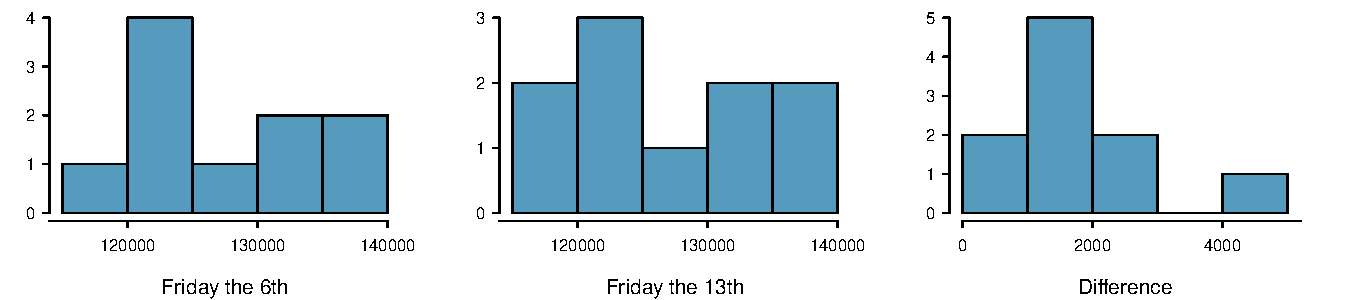
\includegraphics[width=\textwidth]{ch_inference_for_means/figures/eoce/friday_13th_traffic/friday_13th_traffic_hist} \\
$\:$ \\
{\small
\begin{tabular}{l c c c}
\hline
        & 6$^{\text{th}}$   & 13$^{\text{th}}$  & Diff.\\
\hline  
$\bar{x}$   &128,385            & 126,550       & 1,835 \\
$s$     &7,259          & 7,664         & 1,176 \\
$n$     &10             & 10                & 10 \\
\hline
\end{tabular}
}
\end{center}
\begin{parts}
\item Are there any underlying structures in these data that should be 
considered in an analysis? Explain.
\item What are the hypotheses for evaluating whether the number of people out 
on Friday the 6$^{\text{th}}$ is different than the number out on Friday the 
13$^{\text{th}}$?
\item Check conditions to carry out the hypothesis test from part~(b).
\item Calculate the test statistic and the p-value.
\item What is the conclusion of the hypothesis test?
\item Interpret the p-value in this context.
\item What type of error might have been made in the conclusion of your test? 
Explain.
\end{parts}
}{}

% 24

\eoce{\qt{Diamonds, Part I\label{diamonds_1}} Prices of diamonds are determined by 
what is known as the 4 Cs: cut, clarity, color, and carat weight. The prices of 
diamonds go up as the carat weight increases, but the increase is not smooth. 
For example, the difference between the size of a 0.99 carat diamond and a 1 
carat diamond is undetectable to the naked human eye, but the price of a 1 
carat diamond tends to be much higher than the price of a 0.99 diamond. In this 
question we use two random samples of diamonds, 0.99 carats and 1 carat, each 
sample of size 23, and compare the average prices of the diamonds. In order to 
be able to compare equivalent units, we first divide the price for each diamond 
by 100 times its weight in carats. That is, for a 0.99 carat diamond, we divide 
the price by 99. For a 1 carat diamond, we divide the price by 100. The 
distributions and some sample statistics are shown below.\footfullcite{ggplot2} \\[1mm]
\begin{minipage}[c]{0.57\textwidth}
Conduct a hypothesis test to evaluate if there is a difference between the 
average standardized prices of 0.99 and 1 carat diamonds. Make sure to state 
your hypotheses clearly, check relevant conditions, and interpret your results 
in context of the data. \\[2mm]
\begin{tabular}{l c c }
\hline
        & 0.99 carats       & 1 carat\\
\hline  
Mean    & \$44.51          & \$56.81           \\
SD      & \$13.32          &\$16.13            \\
n       &23             & 23 \\
\hline
\end{tabular}
\end{minipage}%
\begin{minipage}[c]{0.43\textwidth}
\begin{center}
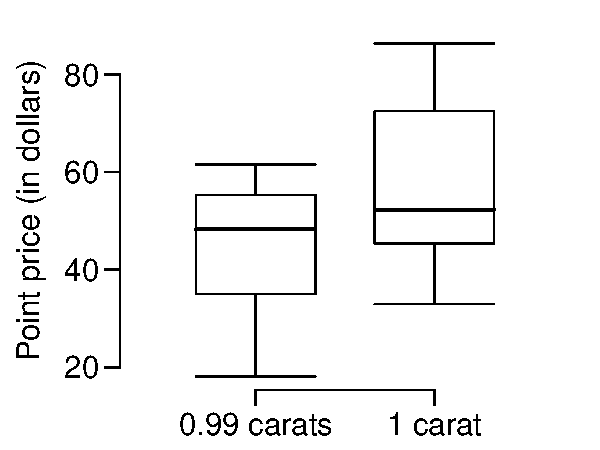
\includegraphics[width=0.875\textwidth]{ch_inference_for_means/figures/eoce/diamonds_1/diamonds_box.pdf}
\end{center}
\end{minipage}
}{}

\D{\newpage}

% 25

\eoce{\qt{Friday the 13$^{\text{th}}$, Part II\label{friday_13th_accident}}
The Friday the $13^{th}$ study reported in
Exercise~\ref{friday_13th_traffic} also provides data on traffic
accident related emergency room admissions.
The distributions of these counts from Friday the 6$^{\text{th}}$ and
Friday the 13$^{\text{th}}$ are shown below for six such paired dates
along with summary statistics.
You may assume that conditions for inference are met.
\begin{center}
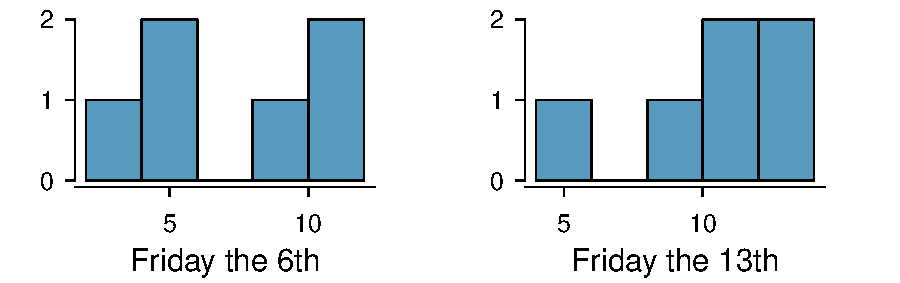
\includegraphics[width=0.9\textwidth]{ch_inference_for_means/figures/eoce/friday_13th_accident/friday_13th_accident_hist} \\
$\:$ \\
\begin{minipage}[c]{0.32\textwidth}
\begin{tabular}{l c c c}
\hline
        & 6$^{\text{th}}$   & 13$^{\text{th}}$  & diff\\
\hline  
Mean    &7.5                & 10.83             & -3.33 \\
SD      &3.33           & 3.6               & 3.01 \\
n       &6              & 6             & 6 \\
\hline
\end{tabular}
\end{minipage}
\end{center}

\begin{parts}
\item Conduct a hypothesis test to evaluate if there is a difference between 
the average numbers of traffic accident related emergency room admissions 
between Friday the 6$^{\text{th}}$ and Friday the~13$^{\text{th}}$.
\item Calculate a 95\% confidence interval for the difference between the 
average numbers of traffic accident related emergency room admissions between 
Friday the 6$^{\text{th}}$ and Friday the 13$^{\text{th}}$.
\item The conclusion of the original study states, ``Friday 13th is unlucky for 
some. The risk of hospital admission as a result of a transport accident may be 
increased by as much as 52\%. Staying at home is recommended.'' Do you agree 
with this statement? Explain your reasoning.
\end{parts}
}{}

% 26

\eoce{\qt{Diamonds, Part II\label{diamonds_2}} In Exercise~\ref{diamonds_1}, we 
discussed diamond prices (standardized by weight) for diamonds with weights 0.
99 carats and 1 carat. See the table for summary statistics, and then construct 
a 95\% confidence interval for the average difference between the standardized 
prices of 0.99 and 1 carat diamonds. You may assume the conditions for 
inference are met.
\begin{center}
\begin{tabular}{l c c }
\hline
        & 0.99 carats       & 1 carat\\
\hline  
Mean    & \$44.51          & \$56.81           \\
SD      & \$13.32          &\$16.13            \\
n       &23             & 23 \\
\hline
\end{tabular}
\end{center}
}{}

% 27

\eoce{\qt{Chicken diet and weight,
    Part I\label{chick_wts_linseed_horsebean}}
Chicken farming is a multi-billion dollar industry,
and any methods that increase the growth rate of young
chicks can reduce consumer costs while increasing
company profits, possibly by millions of dollars.
An experiment was conducted to measure and compare
the effectiveness of various feed supplements on the
growth rate of chickens.
Newly hatched chicks were randomly allocated into six groups, 
and each group was given a different feed supplement.
Below are some summary statistics from this data set along
with box plots showing the distribution of weights by
feed type.\footfullcite{data:chickwts}

\noindent\begin{minipage}[c]{0.65\textwidth}
\begin{center}
\includegraphics[width= \textwidth]{ch_inference_for_means/figures/eoce/chick_wts_linseed_horsebean/chick_wts_box.pdf}
\end{center}
\end{minipage}
\begin{minipage}[c]{0.35\textwidth}
{\footnotesize\begin{tabular}{l c c c}
\hline
            & Mean      & SD        & n \\
\hline
casein          & 323.58        & 64.43 & 12 \\
horsebean   & 160.20        & 38.63 & 10 \\
linseed         & 218.75        & 52.24 & 12 \\
meatmeal    & 276.91        & 64.90 & 11 \\
soybean         & 246.43        & 54.13 & 14 \\
sunflower       & 328.92        & 48.84 & 12 \\
\hline
\end{tabular}}
\end{minipage} 

\begin{parts}
\item Describe the distributions of weights of chickens that were fed linseed 
and horsebean.
\item Do these data provide strong evidence that the average weights of 
chickens that were fed linseed and horsebean are different? Use a 5\% 
significance level.
\item What type of error might we have committed? Explain.
\item Would your conclusion change if we used $\alpha = 0.01$?
\end{parts}
}{}

\D{\newpage}

% 28

\eoce{\qt{Fuel efficiency of manual and automatic cars, Part I\label{fuel_eff_city}} 
Each year the US Environmental Protection Agency (EPA)
releases fuel economy data on cars manufactured in that year.
Below are summary statistics on fuel efficiency (in miles/gallon)
from random samples of cars with manual and automatic transmissions.
Do these data provide strong evidence of a difference between the
average fuel efficiency of cars with manual and automatic
transmissions in terms of their average city mileage?
Assume that conditions for inference are
satisfied. \footfullcite{data:epaMPG}

\noindent\begin{minipage}[c]{0.38\textwidth}
\begin{center}
\begin{tabular}{l c c }
\hline
        & \multicolumn{2}{c}{City MPG} \\
\hline
        & Automatic     & Manual         \\
Mean    & 16.12         & 19.85      \\
SD      & 3.58          & 4.51       \\
n       & 26            & 26 \\
\hline
& \\
& \\
\end{tabular}
\end{center}
\end{minipage}
\begin{minipage}[c]{0.6\textwidth}
\begin{center}
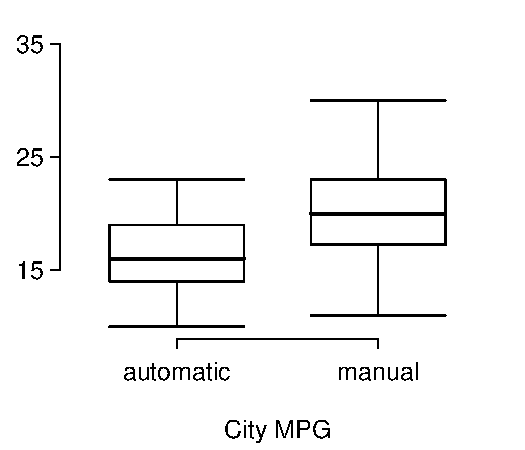
\includegraphics[width=0.7\textwidth]{ch_inference_for_means/figures/eoce/fuel_eff_city/fuel_eff_city_box.pdf}
\end{center}
\end{minipage}
}{}

% 29

\eoce{\qt{Chicken diet and weight, Part II\label{chick_wts_casein_soybean}} Casein is 
a common weight gain supplement for humans. Does it have an effect on chickens? 
Using data provided in Exercise~\ref{chick_wts_linseed_horsebean}, test the 
hypothesis that the average weight of chickens that were fed casein is 
different than the average weight of chickens that were fed soybean. If your 
hypothesis test yields a statistically significant result, discuss whether or 
not the higher average weight of chickens can be attributed to the casein diet. 
Assume that conditions for inference are satisfied.
}{}

% 30

\eoce{\qt{Fuel efficiency of manual and automatic cars, Part II\label{fuel_eff_hway}} 
The table provides summary statistics on highway fuel economy
of the same 52 cars from Exercise~\ref{fuel_eff_city}.
Use these statistics to calculate a 98\% confidence interval
for the difference between average highway mileage of manual
and automatic cars, and interpret this interval in the context
of the data.\footfullcite{data:epaMPG}

\noindent\begin{minipage}[c]{0.38\textwidth}
\begin{center}
\begin{tabular}{l c c }
\hline
        & \multicolumn{2}{c}{Hwy MPG} \\
\hline
            & Automatic     & Manual         \\
Mean    & 22.92         & 27.88          \\
SD      & 5.29          & 5.01           \\
n       & 26            & 26 \\
\hline
& \\
& \\
\end{tabular}
\end{center}
\end{minipage}
\begin{minipage}[c]{0.6\textwidth}
\begin{center}
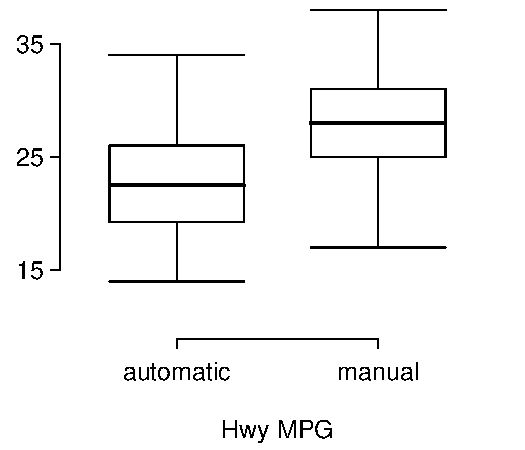
\includegraphics[width=0.7\textwidth]{ch_inference_for_means/figures/eoce/fuel_eff_hway/fuel_eff_hway_box.pdf}
\end{center}
\end{minipage}
}{}

\D{\newpage}

% 31

\eoce{\qt{Prison isolation experiment, Part I\label{prison_isolation_T}}
Subjects from Central Prison in Raleigh, NC, volunteered
for an experiment involving an ``isolation'' experience.
The goal of the experiment was to find a treatment 
that reduces subjects' psychopathic deviant T scores.
This score measures a person's need for control or their rebellion against 
control, and it is part of a commonly used mental health test called the 
Minnesota Multiphasic Personality Inventory (MMPI) test. The experiment had 
three treatment groups: 
\begin{enumerate}[(1)]
\setlength{\itemsep}{0mm}
\item
    Four hours of sensory restriction plus a 15 minute
    ``therapeutic" tape advising that professional help
    is available.
\item
    Four hours of sensory restriction plus a 15 minute
    ``emotionally neutral'' tape on training hunting dogs.
\item
    Four hours of  sensory restriction but no taped message.
\end{enumerate}
Forty-two subjects were randomly assigned to these treatment groups, and an 
MMPI test was administered before and after the treatment. Distributions of the 
differences between pre and post treatment scores (pre - post) are shown below, 
along with some sample statistics. Use this information to independently test 
the effectiveness of each treatment. Make sure to clearly state your 
hypotheses, check conditions, and interpret results in the context of the data.\footfullcite{data:prison}

\begin{center}
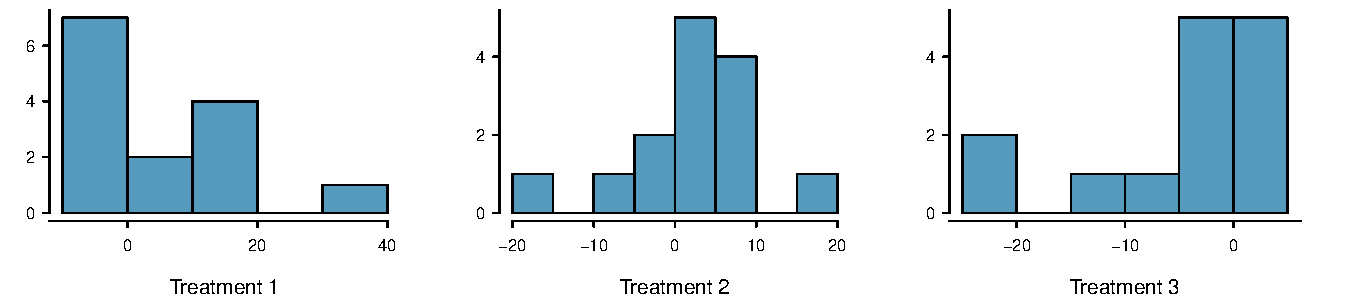
\includegraphics[width=\textwidth]{ch_inference_for_means/figures/eoce/prison_isolation_T/prison_isolation_hist} \\
$\:$ \\
\begin{tabular}{l  r  r  r  r  }
\hline
                & Tr 1  & Tr 2  & Tr 3      \\
\hline
Mean            & 6.21  & 2.86  & -3.21           \\
SD              & 12.3  & 7.94  & 8.57       \\
n               & 14        & 14        & 14     \\
\hline
\end{tabular}
\end{center}
}{}

% 32

\eoce{\qt{True / False: comparing means\label{tf_compare_means}} Determine if the 
following statements are true or false, and explain your reasoning for 
statements you identify as false.
\begin{parts}
\item When comparing means of two samples where $n_1 = 20$ and $n_2 = 40$, we 
can use the normal model for the difference in means since $n_2 \ge 30$.
\item As the degrees of freedom increases, the $t$-distribution approaches 
normality.
\item We use a pooled standard error for calculating the standard error of the 
difference between means when sample sizes of groups are equal to each other.
\end{parts}
}{}
}







%__________________
\section{Power calculations for a difference of means}
\label{PowerForDifferenceOfTwoMeans}

\noindent%
Often times in experiment planning,
there are two competing considerations:
\begin{itemize}
\setlength{\itemsep}{0mm}
\item
    We want to collect enough data that we can detect
    important effects.
\item
    Collecting data can be expensive, and in experiments
    involving people, there may be some risk to patients.
\end{itemize}
In this section, we focus on the context of a clinical trial,
which is a health-related experiment where the subject
are people, and we will determine an appropriate sample size
where we can be 80\% sure that we would detect any practically
important effects.\footnote{Even though we don't cover it
  explicitly, similar sample size planning is also helpful
  for observational studies.}


\subsection{Going through the motions of a test}

We're going to go through the motions of a hypothesis test.
This will help us frame our calculations for determining
an appropriate sample size for the study.

\begin{examplewrap}
\begin{nexample}{Suppose a pharmaceutical company has developed
    a new drug for lowering blood pressure, and they are
    preparing a clinical trial (experiment) to test the
    drug's effectiveness.
    They recruit people who are taking a particular standard
    blood pressure medication.
    People in the control group will continue to take their
    current medication through generic-looking pills to ensure
    blinding.
    Write down the hypotheses for a two-sided hypothesis test
    in this context.}
  Generally, clinical trials use a two-sided alternative
  hypothesis, so below are suitable hypotheses for this context:
  \begin{description}
  \setlength{\itemsep}{0mm}
  \item[$H_0$:]
      The new drug performs exactly as well as the
      standard medication. \\
      $\mu_{trmt} - \mu_{ctrl} = 0$.
  \item[$H_A$:]
      The new drug's performance differs from the
      standard medication. \\
      $\mu_{trmt} - \mu_{ctrl} \neq 0$.
  \end{description}
%  This two-sided test ensures we'll be alerted if either
%  the new drug works better or worse than the standard
%  medication.
\end{nexample}
\end{examplewrap}

\begin{examplewrap}
\begin{nexample}{The researchers would like to run the clinical
    trial on patients with systolic blood pressures between 140
    and 180~mmHg.
    Suppose previously published studies suggest that the
    standard deviation of the patients' blood pressures will
    be about 12~mmHg and the distribution of patient blood
    pressures will be approximately symmetric.\footnotemark{}
    If~we had 100 patients per group, what would be the
    approximate standard error for
    $\bar{x}_{trmt} - \bar{x}_{ctrl}$?}
  The standard error is calculated as follows:
  \begin{align*}
  SE_{\bar{x}_{trmt} - \bar{x}_{ctrl}}
    = \sqrt{\frac{s_{trmt}^2}{n_{trmt}} +
        \frac{s_{ctrl}^2}{n_{ctrl}}}
    = \sqrt{\frac{12^2}{100} + \frac{12^2}{100}}
    = 1.70
  \end{align*}
  This may be an imperfect estimate of
  $SE_{\bar{x}_{trmt} - \bar{x}_{ctrl}}$,
  since the standard deviation estimate we used may not
  be perfectly correct for this group of patients.
  However, it is sufficient for our purposes.
\end{nexample}
\end{examplewrap}
\footnotetext{In this particular study, we'd generally measure
  each patient's blood pressure at the beginning and end
  of the study, and then the outcome measurement for
  the study would be the average change in blood pressure.
  That is, both $\mu_{trmt}$ and $\mu_{ctrl}$ would
  represent average differences.
  This is what you might think of as a 2-sample paired
  testing structure, and we'd analyze it exactly just like
  a hypothesis test for a difference in the average change
  for patients.
  In the calculations we perform here, we'll suppose
  that 12~mmHg is the predicted standard deviation of
  a patient's blood pressure difference over the course
  of the study.}

\begin{examplewrap}
\begin{nexample}{What does the null distribution of
    $\bar{x}_{trmt} - \bar{x}_{ctrl}$ look like?}
  The degrees of freedom are greater than 30, so the
  distribution of $\bar{x}_{trmt} - \bar{x}_{ctrl}$
  will be approximately normal.
  The standard deviation of this distribution
  (the standard error) would be about 1.70, and under
  the null hypothesis, its mean would be 0.
  \begin{center}
  \Figures{0.93}{power_null_0_1-7}{power_null_A_0_1-7}
  \end{center}
\end{nexample}
\end{examplewrap}

\begin{examplewrap}
\begin{nexample}{For what values of
    $\bar{x}_{trmt} - \bar{x}_{ctrl}$ would we reject
    the null hypothesis?}
  For $\alpha = 0.05$, we would reject $H_0$ if the difference
  is in the lower 2.5\% or upper 2.5\% tail:
  \begin{description}
  \setlength{\itemsep}{0mm}
  \item[Lower 2.5\%:]
      For the normal model, this is 1.96 standard errors
      below~0, so any difference smaller than
      $-1.96 \times 1.70 = -3.332$~mmHg.
  \item[Upper 2.5\%:]
      For the normal model, this is 1.96 standard errors
      above~0, so any difference larger than
      $1.96 \times 1.70 = 3.332$~mmHg.
  \end{description}
  The boundaries of these \term{rejection regions} are shown below:
  \begin{center}
  \Figures{0.93}{power_null_0_1-7}
      {power_null_B_0_1-7_with_rejection_region}
  \end{center}
\end{nexample}
\end{examplewrap}

Next, we'll perform some hypothetical calculations to determine
the probability we reject the null hypothesis, if the alternative
hypothesis were actually true.


\subsection%[Computing the power for a 2-sample test]
    {Computing the power for a 2-sample test}

When planning a study, we want to know how likely we are
to detect an effect we care about.
In~other words, if there is a real effect, and that effect
is large enough that it has practical value, then what's
the probability that we detect that effect?
This probability is called the \term{power}, and we can
compute it for different sample sizes or for different
\emph{effect sizes}.

We first determine what is a practically significant result.
Suppose that the company researchers care about finding any
effect on blood pressure that is 3~mmHg or larger vs the
standard medication.
Here, 3~mmHg is the minimum \term{effect size} of interest,
and we want to know how likely we are to detect this size
of an effect in the study.

\begin{examplewrap}
\begin{nexample}{Suppose we decided to move forward with
    100 patients per treatment group and the new drug reduces
    blood pressure by an additional 3~mmHg relative to the
    standard medication.
    What is the probability that we detect a drop?}
  \label{PowerFor100AtNeg3}%
  Before we even do any calculations, notice that if
  $\bar{x}_{trmt} - \bar{x}_{ctrl} = -3$~mmHg, there
  wouldn't even be sufficient evidence to reject $H_0$.
  That's not a good sign.

  To calculate the probability that we will reject $H_0$,
  we need to determine a few things:
  \begin{itemize}
  \setlength{\itemsep}{0mm}
  \item
      The sampling distribution for
      $\bar{x}_{trmt} - \bar{x}_{ctrl}$ when the true difference
      is -3~mmHg.
      This is the same as the null distribution,
      except it is shifted to the left by~3:
      \begin{center}
      \Figures{0.87}{power_null_0_1-7}
          {power_null_C_0_1-7_with_alt_at_3}
      \end{center}
  \item
      The rejection regions, which are outside of the
      dotted lines above.
  \item
      The fraction of the distribution that falls in the
      rejection region.
  \end{itemize}
  In short, we need to calculate the probability that
  $x < -3.332$ for a normal distribution with mean -3
  and standard deviation~1.7.
  To do so, we first shade the area we want to calculate:
  \begin{center}
    \Figures{0.93}{power_null_0_1-7}
        {power_null_D_0_1-7_with_alt_at_3_and_shaded}
  \end{center}
  We'll use a normal approximation, which is good approximation
  when the degrees of freedom is about 30 or more.
  We'll start by calculating the Z-score and find the tail area
  using either statistical software or the probability table:
  \begin{align*}
  Z = \frac{-3.332 - (-3)}{1.7} = -0.20 \qquad \to \qquad 0.42
  \end{align*}
  The power for the test is about 42\% when
  $\mu_{trmt} - \mu_{ctrl} = -3$ and each group has
  a sample size of~100.
\end{nexample}
\end{examplewrap}

In Example~\ref{PowerFor100AtNeg3}, we ignored the upper
rejection region in the calculation, which was in the
opposite direction of the hypothetical truth, i.e. -3.
The reasoning?
There wouldn't be any value in rejecting the null hypothesis
and concluding there was an increase when in fact there was
a decrease.

We've also used a normal distribution instead
of the $t$-distribution.
This is a convenience, and if the sample size is too small,
we'd need to revert back to using the $t$-distribution.
We'll discuss this a bit further at the end of this section.


\D{\newpage}

\subsection{Determining a proper sample size}

In the last example, we found that if we have a sample size
of 100 in each group, we can only detect an effect size of
3~mmHg with a probability of about 0.42.
Suppose the researchers moved forward and only used
100 patients per group, and the data did not support
the alternative hypothesis,
i.e. the researchers did not reject $H_0$.
This is a very bad situation to be in for a few reasons:
\begin{itemize}
\setlength{\itemsep}{0mm}
\item
    In the back of the researchers' minds, they'd all be
    wondering, \emph{maybe there is a real and meaningful
    difference, but we weren't able to detect it with such
    a small sample}. 
\item
    The company probably invested hundreds of millions
    of dollars in developing the new drug, so now they
    are left with great uncertainty about its potential
    since the experiment didn't have a great shot at
    detecting effects that could still be important.
\item
    Patients were subjected to the drug, and we can't even
    say with much certainty that the drug doesn't help
    (or harm) patients.
\item
    Another clinical trial may need to be run to get a more
    conclusive answer as to whether the drug does hold any
    practical value, and conducting a second clinical trial
    may take years and many millions of dollars.
\end{itemize}
We want to avoid this situation, so we need to determine
an appropriate sample size to ensure we can be pretty
confident that we'll detect any effects that are practically
important.
As mentioned earlier, a change of 3~mmHg was deemed to be the
minimum difference that was practically important.
As~a first step, we could calculate power for several
different sample sizes.
For instance, let's try 500 patients per group.

\begin{exercisewrap}
\begin{nexercise}
Calculate the power to detect a change of -3~mmHg when using
a sample size of 500 per group.\footnotemark{}
\begin{enumerate}[(a)]
\setlength{\itemsep}{0mm}
\item
    Determine the standard error (recall that the standard
    deviation for patients was expected to be about 12~mmHg).
\item
    Identify the null distribution and rejection regions.
\item
    Identify the alternative distribution when
    $\mu_{trmt} - \mu_{ctrl} = -3$.
\item
    Compute the probability we reject the null hypothesis.
\end{enumerate}
\end{nexercise}
\end{exercisewrap}
\footnotetext{(a) The standard error is given as
  $SE = \sqrt{\frac{12^2}{500} + \frac{12^2}{500}} = 0.76$.\\
  (b)~\&~(c)~The null distribution, rejection boundaries,
  and alternative distribution are shown below: \\
  \indent%
  \Figures{0.7}{power_null_0_0-76}
      {power_null_0_0-76_with_alt_at_3_and_shaded} \\
  The rejection regions are the areas on the outside of the
  two dotted lines and are at $\pm 0.76 \times 1.96 = \pm 1.49$. \\
  (d)~The area of the alternative distribution where
  $\mu_{trmt} - \mu_{ctrl} = -3$ has been shaded.
  We compute the Z-score and find the tail area:
  $Z = \frac{-1.49 - (-3)}{0.76} = 1.99 \to 0.977$.
%  (can use $df = 500$ from the minimum of the two sample
%  sizes minus 1),
%  which is the power of the test for a difference of 3~mmHg.
  With 500 patients per group, we would be about 97.7\% sure
  (or~more) that we'd detect any effects that are at least
  3~mmHg in size.}

The researchers decided 3~mmHg was the minimum difference
that was practically important, and with a sample size of~500,
we can be very certain (97.7\% or better) that we will detect
any such difference.
We now have moved to another extreme where we are exposing
an unnecessary number of patients to the new drug in the
clinical trial.
Not only is this ethically questionable, but it would also
cost a lot more money than is necessary to be quite sure
we'd detect any important effects.

The most common practice is to identify the sample size where
the power is around 80\%, and sometimes 90\%.
Other values may be reasonable for a specific context,
but 80\% and 90\% are most commonly targeted as a good
balance between high power and not exposing too many
patients to a new treatment (or wasting too much money).

We could compute the power of the test at several other
possible sample sizes until we find one that's close to~80\%,
but there's a better way.
We should solve the problem backwards.

\begin{examplewrap}
\begin{nexample}{What sample size will lead to a power of 80\%?}
  \label{sample_size_for_80_percent_power}%  This is referenced in EOCE.
  We'll assume we have a large enough sample that the normal
  distribution is a good approximation for the test statistic,
  since the normal distribution and the $t$-distribution
  look almost identical when the degrees of freedom are
  moderately large (e.g. $df \geq 30$).
  If that doesn't turn out to be true, then we'd need to make
  a correction.

  We start by identifying the Z-score that would give us a lower
  tail of 80\%.
  For a moderately large sample size per group,
  the Z-score for a lower tail of 80\% would be about $Z = 0.84$.
%  (If our calculations suggest a very sample size,
%  we should recalculate this part and basically do the
%  problem one more time.)
  \begin{center}
    \Figure{0.93}{power_best_sample_size}
  \end{center}
  Additionally, the rejection region extends
  $1.96\times SE$ from the center of the null distribution
  for $\alpha = 0.05$.
  This allows us to calculate the target distance between
  the center of the null and alternative distributions in
  terms of the standard error:
  \begin{align*}
  0.84 \times SE + 1.96 \times SE = 2.8 \times SE
  \end{align*}
  In our example, we want the distance between the null
  and alternative distributions' centers to equal the minimum
  effect size of interest, 3~mmHg, which allows us to set up
  an equation between this difference and the standard error:
  \begin{align*}
  3 &= 2.8 \times SE \\
  3 &= 2.8 \times \sqrt{\frac{12^2}{n} + \frac{12^2}{n}} \\
  n &= \frac{2.8^2}{3^2} \times \left( 12^2 + 12^2 \right)
    = 250.88 \\
  \end{align*}
  We should target 251 patients per group in order to achieve
  80\% power at the 0.05 significance level for this context.
\end{nexample}
\end{examplewrap}

The standard error difference of $2.8 \times SE$ is specific
to a context where the targeted power is 80\% and the
significance level is $\alpha = 0.05$.
If the targeted power is 90\% or if we use a different
significance level, then we'll use something a little
different than $2.8 \times SE$.

Had the suggested sample size been relatively small
-- roughly 30 or smaller -- it would have been a good idea
to rework the calculations using the degrees of fredom
for the smaller sample size under that initial sample size.
That is, we would have revised the 0.84 and 1.96
values based on degrees of freedom implied by the initial
sample size.
The revised sample size target would generally have then
been a little larger.

%\begin{examplewrap}
%\begin{nexample}{Suppose the suggested sample size from
%    the power calculation was 15 per group.
%    This is a relatively small sample size,
%    and the conditions about the sample size being
%    large in Example~\ref{}
%    wouldn't be valid.
%    What should we do?}
%  First, recognizing that there is \emph{something}
%  to do is already great here:
%  it's easy to forget the earlier assumption about
%  a moderately large sample size.
%  So if you catch yourself here, that is something
%  to be commended!
%
%  Next, we basically update the values of 0.84 and 1.96
%  in the calculations.
%  First, we identify the degrees of freedom
%  ($df = 14$ as a rough guide, though 
%  We'd find the values
%  corresponding to this more precise $t$-distribution.
%  For example, had the sample-size per group been suggested
%  as~15, we would have used $df = 14$;
%  this would have led to a T-score of 0.87 (in place of 0.84)
%  and a rejection region cutoff of 2.14.
%  The reworked sample size would then have been suggested
%  as about 16\% larger.
%  If we did not do this extra step, our estimated power would
%  drop from 80\% to 74\%.
%  While that would not be the end of the world, being precise
%  is part of the job of being a data scientist!
%\end{nexample}
%\end{examplewrap}

\D{\newpage}

\begin{exercisewrap}
\begin{nexercise}
Suppose the targeted power was 90\% and we were using
$\alpha = 0.01$.
How many standard errors should separate the centers
of the null and alternative distribution, where the
alternative distribution is centered at the minimum
effect size of interest?\footnotemark{}
\end{nexercise}
\end{exercisewrap}
\footnotetext{First, find the Z-score such that 90\% of the
  distribution is below it: $Z = 1.28$.
  Next, find the cutoffs for the rejection regions: $\pm 2.58$.
  Then the difference in centers should be about
  $1.28 \times SE + 2.58 \times SE = 3.86 \times SE$.}

\begin{exercisewrap}
\begin{nexercise}
What are some considerations that are important in determining
what the power should be for an experiment?\footnotemark{}
\end{nexercise}
\end{exercisewrap}
\footnotetext{Answers will vary, but here are a few
  important considerations:
  \begin{itemize}
  \setlength{\itemsep}{0mm}
  \item Whether there is any risk to patients in the study.
  \item The cost of enrolling more patients.
  \item The potential downside of not detecting an effect
      of interest.
  \end{itemize}}

Figure~\ref{power_curve_neg-3} shows the power for sample
sizes from 20~patients to 5,000~patients when $\alpha = 0.05$
and the true difference is -3.
This curve was constructed by writing a program to compute
the power for many different sample sizes.

\begin{figure}[h]
  \centering
  \Figures{0.9}{power_curve}{power_curve_neg-3}
  \caption{The curve shows the power for different sample
      sizes in the context of the blood pressure example when
      the true difference is~-3.
      Having more than about 250 to 350 observations doesn't
      provide much additional value in detecting an effect when
      $\alpha = 0.05$.}
  \label{power_curve_neg-3}
\end{figure}

%\begin{exercisewrap}
%\begin{nexercise}
%
%\end{nexercise}
%\end{exercisewrap}

Power calculations for expensive or risky experiments are
critical.
However, what about experiments that are inexpensive and
where the ethical considerations are minimal?
For example, if we are doing final testing on a new feature
on a popular website, how would our sample size considerations
change?
As before, we'd want to make sure the sample is big enough.
However, suppose the feature has undergone some testing and
is known to perform well
(e.g.~the website's users seem to enjoy the feature).
Then it may be reasonable to run a larger experiment
if there's value from having a more precise estimate
of the feature's effect, such as helping guide the
development of the next useful feature.


{\exercisesheader{}

% 33

\eoce{\qt{Increasing corn yield\label{increase_corn_yield}} A large farm wants to 
try out a new type of fertilizer to evaluate whether it will improve the 
farm's corn production. The land is broken into plots that produce an 
average of 1,215 pounds of corn with a standard deviation of 94 pounds per 
plot. The owner is interested in detecting any average difference of at 
least 40 pounds per plot. How many plots of land would be needed for the 
experiment if the desired power level is 90\%? Assume each plot of land gets 
treated with either the current fertilizer or the new fertilizer.
}{}

% 34

\eoce{\qt{Email outreach efforts\label{email_outreach_efforts}} A medical research 
group is recruiting people to complete short surveys about their medical 
history. For example, one survey asks for information on a person's family 
history in regards to cancer. Another survey asks about what topics were 
discussed during the person's last visit to a hospital. So far, as people 
sign up, they complete an average of just 4~surveys, and the standard 
deviation of the number of surveys is about~2.2. The research group wants to 
try a new interface that they think will encourage new enrollees to complete 
more surveys, where they will randomize each enrollee to either get the new 
interface or the current interface. How many new enrollees do they need for 
each interface to detect an effect size of 0.5 surveys per enrollee, if the 
desired power level is 80\%?
}{}
}





%__________________
\section{Comparing many means with ANOVA}
\label{anovaAndRegrWithCategoricalVariables}

\index{analysis of variance (ANOVA)|(}

\noindent%
Sometimes we want to compare means across many groups.
We might initially think to do pairwise comparisons.
For example, if there were three groups, we might be tempted
to compare the first mean with the second,
then with the third,
and then finally compare the second and third means for
a total of three comparisons.
However, this strategy can be treacherous.
If we have many groups and do many comparisons,
it is likely that we will eventually find a difference
just by chance, even if there is no difference in the
populations.
Instead, we should apply a holistic test to check whether
there is evidence that at least one pair groups are
in fact different, and this is where \emph{ANOVA} saves
the~day.


\subsection{Core ideas of ANOVA}

In this section, we will learn a new method called
\term{analysis of variance (ANOVA)} and a new test
statistic called $F$.
ANOVA uses a single hypothesis test to check whether
the means across many groups are equal:
\begin{itemize}
\setlength{\itemsep}{0mm}
\item[$H_0$:] The mean outcome is the same across all groups. In statistical notation, $\mu_1 = \mu_2 = \cdots = \mu_k$ where $\mu_i$ represents the mean of the outcome for observations in category $i$.
\item[$H_A$:] At least one mean is different.
\end{itemize}
Generally we must check three conditions on the data before performing ANOVA:
\begin{itemize}
\setlength{\itemsep}{0mm}
\item the observations are independent within and across groups,
\item the data within each group are nearly normal, and
\item the variability across the groups is about equal.
\end{itemize}
When these three conditions are met, we may perform an ANOVA to determine whether the data provide strong evidence against the null hypothesis that all the $\mu_i$ are equal.

\begin{examplewrap}
\begin{nexample}{College departments commonly run multiple
    lectures of the same introductory course each semester
    because of high demand.
    Consider a statistics department that runs three lectures
    of an introductory statistics course.
    We might like to determine whether there are statistically
    significant differences in first exam scores in these three
    classes ($A$,~$B$, and~$C$).
    Describe appropriate hypotheses to determine whether
    there are any differences between the three classes.}
  \label{firstExampleForThreeStatisticsClassesAndANOVA}%
  The hypotheses may be written in the following form:
  \begin{itemize}
  \setlength{\itemsep}{0mm}
  \item[$H_0$:]
      The average score is identical in all lectures.
      Any observed difference is due to chance.
      Notationally, we write $\mu_A=\mu_B=\mu_C$.
  \item[$H_A$:]
      The average score varies by class.
      We would reject the null hypothesis in favor of the
      alternative hypothesis if there were larger differences
      among the class averages than what we might expect
      from chance alone.
  \end{itemize}
\end{nexample}
\end{examplewrap}

Strong evidence favoring the alternative hypothesis in ANOVA
is described by unusually large differences among the group means.
We will soon learn that assessing the variability of the group
means relative to the variability among individual observations
within each group is key to ANOVA's success.

\begin{examplewrap}
\begin{nexample}{Examine Figure~\ref{toyANOVA}.
    Compare groups I, II, and III.
    Can you visually determine if the differences in the group
    centers is due to chance or not? Now compare
    groups IV, V, and~VI.
    Do these differences appear to be due to chance?}
  Any real difference in the means of groups I, II, and~III
  is difficult to discern, because the data within each group
  are very volatile relative to any differences in the
  average outcome.
  On the other hand, it appears there are differences
  in the centers of groups IV, V, and~VI.
  For instance, group~V appears to have a higher mean than
  that of the other two groups.
  Investigating groups IV, V, and~VI, we see the differences
  in the groups' centers are noticeable because those
  differences are large \emph{relative to the variability
  in the individual observations within each group}.
\end{nexample}
\end{examplewrap}

\begin{figure}[h]
  \centering
  \Figure{0.68}{toyANOVA}
  \caption{Side-by-side dot plot for the outcomes for six groups.}
  \label{toyANOVA}
\end{figure}


\subsection{Is batting performance related to player position in MLB?}

\index{data!MLB batting|(}

\newcommand{\mlbdata}{\data{bat18}}
\newcommand{\mlbN}{429}
\newcommand{\mlbK}{3}
\newcommand{\mlbMinAB}{100}
\newcommand{\mlbDFA}{2}
\newcommand{\mlbDFB}{426}
\newcommand{\mlbF}{5.077}
\newcommand{\mlbPvalue}{0.0066}

We would like to discern whether there are real differences
between the batting performance of baseball players according
to their position:
outfielder (\resp{OF}), infielder (\resp{IF}),
%designated hitter (\resp{DH}),
and catcher (\resp{C}).
We will use a data set called \mlbdata{},
which includes batting records of \mlbN{} Major League
Baseball (MLB) players from the 2018 season who had
at least \mlbMinAB{} at bats.
Six of the \mlbN{} cases represented in \mlbdata{}
are shown in Figure~\ref{mlbBat18DataMatrix},
and descriptions for each variable are provided
in Figure~\ref{mlbBat18Variables}.
The measure we will use for the player batting
performance (the outcome variable) is on-base
percentage (\var{OBP}).
The on-base percentage roughly represents the fraction
of the time a player successfully gets on base or hits
a home run.

\begin{figure}[h]
\centering
\begin{tabular}{r lll ccc ccc}
  \hline
  & name & team & position & AB & H & HR &RBI & AVG & OBP \\ 
  \hline
  1 &  Abreu, J & CWS & IF &  499 &  132 &   22 &
      78 & 0.265 & 0.325 \\
  2 &  Acuna Jr., R & ATL & OF &  433 &  127 &   26 &
      64 & 0.293 & 0.366 \\
  3 &  Adames, W & TB & IF &  288 &   80 &   10 &
      34 & 0.278 & 0.348 \\
  $\vdots$ & $\vdots$ & $\vdots$ & $\vdots$ & $\vdots$ &
      $\vdots$ & $\vdots$ & $\vdots$ \\
  427 &  Zimmerman, R & WSH & IF & 288 &   76 &
      13 &   51 & 0.264 & 0.337 \\
  428 & Zobrist, B & CHC & IF & 455 & 139 & 9 &
      58 & 0.305 & 0.378 \\
  \mlbN{} &  Zunino, M & SEA & C &  373 &   75 &   20 &
      44 & 0.201 & 0.259 \\
   \hline
\end{tabular}
\caption{Six cases from the \mlbdata{} data matrix.}
\label{mlbBat18DataMatrix}
\end{figure}

\begin{figure}[h]
\centering\small
\begin{tabular}{lp{8.5cm}}
\hline
{\bf variable} & {\bf description} \\
\hline
\var{name} & Player name \\
\var{team} & The abbreviated name of the player's team \\
\var{position} &
    The player's primary field position
    (\resp{OF}, \resp{IF}, \resp{C}) \\
\var{AB} & Number of opportunities at bat \\
\var{H} & Number of hits \\
\var{HR} & Number of home runs \\
\var{RBI} & Number of runs batted in \\
\var{AVG} &
    Batting average, which is equal to $\resp{H}/\resp{AB}$ \\
\var{OBP} &
    On-base percentage, which is roughly equal to the fraction
    of times a player gets on base or hits a home run \\
\hline
\end{tabular}
\caption{Variables and their descriptions for the
    \mlbdata{} data set.}
\label{mlbBat18Variables}
\end{figure}

\begin{exercisewrap}
\begin{nexercise}
\label{nullHypForOBPAgainstPosition}%
The null hypothesis under consideration is the following:
$\mu_{\resp{OF}} = \mu_{\resp{IF}} = %\mu_{\resp{DH}} = 
    \mu_{\resp{C}}$.
Write the null and corresponding alternative hypotheses
in plain language.\footnotemark{}
\end{nexercise}
\end{exercisewrap}
\footnotetext{$H_0$: The average on-base percentage is equal
  across the four positions.
  $H_A$: The average on-base percentage varies across some
  (or all) groups.}

\begin{examplewrap}
\begin{nexample}{The player positions have been divided
    into four groups: outfield (\resp{OF}), infield (\resp{IF}),
    %designated hitter (\resp{DH}),
    and catcher~(\resp{C}).
    What would be an appropriate point estimate of the on-base
    percentage by outfielders, $\mu_{\resp{OF}}$?}
  A good estimate of the on-base percentage by outfielders would
  be the sample average of \var{OBP} for just those players
  whose position is outfield: $\bar{x}_{OF} = 0.320$.
\end{nexample}
\end{examplewrap}

Figure~\ref{mlbHRPerABSummaryTable} provides summary statistics for each group. A side-by-side box plot for the on-base percentage is shown in Figure~\ref{mlbANOVABoxPlot}. Notice that the variability appears to be approximately constant across groups; nearly constant variance across groups is an important assumption that must be satisfied before we consider the ANOVA approach.

\begin{figure}[h]
\centering\small
\begin{tabular}{l rrr}
\hline
	& \resp{OF} & \resp{IF} & \resp{C} \\
\hline
Sample size ($n_i$) & 160 & 205 & 64 \\
Sample mean ($\bar{x}_i$) & 0.320 & 0.318 & 0.302 \\
Sample SD ($s_i$) & 0.043 & 0.038 & 0.038 \\
\hline
\end{tabular}
\caption{Summary statistics of on-base percentage, split by player position.}
\label{mlbHRPerABSummaryTable}
\end{figure}

\begin{figure}[h]
  \centering
  \Figures{0.6}{mlbANOVA}{mlbANOVABoxPlot}
  \caption{Side-by-side box plot of the on-base percentage
      for \mlbN{} players across four groups.
      There is one prominent outlier visible in the infield
      group, but with 154 observations in the infield group,
      this outlier is not a concern.}
  \label{mlbANOVABoxPlot}
\end{figure}

\D{\newpage}

\begin{examplewrap}
\begin{nexample}{The largest difference between the sample means
    is between the catcher and the outfielder positions.
    Consider again the original hypotheses:
    \begin{itemize}
    \setlength{\itemsep}{0mm}
    \item[$H_0$:]
        $\mu_{\resp{OF}} = \mu_{\resp{IF}} = \mu_{\resp{C}}$
    \item[$H_A$:]
        The average on-base percentage ($\mu_i$) varies
        across some (or all) groups.
    \end{itemize}
    Why might it be inappropriate to run the test by simply
    estimating whether the difference of $\mu_{\var{C}}$ and
    $\mu_{\resp{OF}}$ is statistically significant at a 0.05
    significance level?}
  \label{multCompExIncDiscOfClassrooms}%
  The primary issue here is that we are inspecting the data
  before picking the groups that will be compared.
  It is inappropriate to examine all data by eye
  (informal testing) and only afterwards decide which parts
  to formally test.
  This is called \term{data snooping} or \term{data fishing}.
  Naturally, we would pick the groups with the large
  differences for the formal test, and this would leading
  to an inflation in the Type~1 Error rate.
  To understand this better, let's consider a slightly
  different problem.

  Suppose we are to measure the aptitude for students in
  20~classes in a large elementary school at the beginning
  of the year.
  In this school, all students are randomly assigned to
  classrooms, so any differences we observe between the
  classes at the start of the year are completely due
  to chance.
  However, with so many groups, we will probably observe
  a few groups that look rather different from each other.
  If we select only these classes that look so different
  and then perform a formal test,
  we will probably make the wrong conclusion that the
  assignment wasn't random.
  While we might only formally test differences
  for a few pairs of classes, we informally evaluated
  the other classes by eye before choosing the most extreme
  cases for a comparison.
\end{nexample}
\end{examplewrap}

For additional information on the ideas expressed in
Example~\ref{multCompExIncDiscOfClassrooms}, we recommend
reading about the
\term{prosecutor's fallacy}.\footnote{See, for example,
  \oiRedirect{textbook-prosecutors_fallacy}
      {andrewgelman.com/2007/05/18/the\_prosecutors}.}

In the next section we will learn how to use the $F$~statistic
and ANOVA to test whether observed differences in sample means
could have happened just by chance even if there was no
difference in the respective population means.


\D{\newpage}

\subsection{Analysis of variance (ANOVA)
    and the $\pmb{F}$-test}

The method of analysis of variance in this context focuses
on answering one question:
is the variability in the sample means so large that it seems
unlikely to be from chance alone?
This question is different from earlier testing procedures
since we will \emph{simultaneously} consider many groups,
and evaluate whether their sample means differ more than
we would expect from natural variation.
We~call this variability the
\term{mean square between groups ($MSG$)},
and it has an associated degrees of freedom,
$df_{G} = k - 1$ when there are
$k$~groups.\index{degrees of freedom (df)!ANOVA}
The $MSG$ can be thought of as a scaled variance formula
for means.
If the null hypothesis is true, any variation in the sample
means is due to chance and shouldn't be too large.
Details of $MSG$ calculations are provided in the
footnote.\footnote{Let $\bar{x}$ represent the mean of
  outcomes across all groups.
  Then the mean square between groups is computed as
  \begin{align*}
  MSG
    = \frac{1}{df_{G}}SSG
    = \frac{1}{k-1}\sum_{i=1}^{k} n_{i}
        \left(\bar{x}_{i} - \bar{x}\right)^2
  \end{align*}
  where $SSG$ is called the \term{sum of squares between groups}
  and $n_{i}$ is the sample size of group $i$.}
However, we typically use software for these computations.

The mean square between the groups is, on its own, quite useless
in a hypothesis test.
We~need a benchmark value for how much variability should
be expected among the sample means if the null hypothesis is true.
To this end, we compute a pooled variance estimate,
often abbreviated as the \term{mean square error ($MSE$)},
which has an associated degrees of freedom value $df_E = n - k$.
It is helpful to think of $MSE$ as a measure of the variability
within the groups.
Details of the computations of the $MSE$ and a link to an
extra online section for ANOVA calculations are provided
in the footnote\footnote{Let $\bar{x}$ represent the mean
  of outcomes across all groups.
  Then the \term{sum of squares total ($SST$)} is computed as
  \begin{align*}
  SST = \sum_{i=1}^{n} \left(x_{i} - \bar{x}\right)^2
  \end{align*}
  where the sum is over all observations in the data set.
  Then we compute the \term{sum of squared errors ($SSE$)}
  in one of two equivalent ways:
  \begin{align*}
  SSE &= SST - SSG \\
  	&= (n_1-1)s_1^2 + (n_2-1)s_2^2 + \cdots + (n_k-1)s_k^2
  \end{align*}
  where $s_i^2$ is the sample variance (square of the standard
  deviation) of the residuals in group $i$.
  Then the $MSE$ is the standardized form of $SSE$:
  $MSE = \frac{1}{df_{E}}SSE$.
  
  \noindent%
  For additional details on ANOVA calculations, see
  \oiRedirect{stat_extra_anova_calculations}
      {www.openintro.org/d?file=stat\_extra\_anova\_calculations}}
for interested readers.

When the null hypothesis is true, any differences among the
sample means are only due to chance, and the $MSG$ and $MSE$
should be about equal.
As~a test statistic for ANOVA, we examine the fraction of $MSG$
and~$MSE$:
\begin{align*}
F = \frac{MSG}{MSE}
\end{align*}
The $MSG$ represents a measure of the between-group variability,
and $MSE$ measures the variability within each of the groups.

\begin{exercisewrap}
\begin{nexercise}
For the baseball data, $MSG = 0.00803$ and $MSE=0.00158$.
Identify the degrees of freedom associated with MSG and
MSE and verify the $F$ statistic is approximately
\mlbF{}.\footnotemark{}
\end{nexercise}
\end{exercisewrap}
\footnotetext{There are $k = \mlbK{}$ groups,
  so $df_{G} = k - 1 = \mlbDFA{}$.
  There are $n = n_1 + n_2 + n_3 = \mlbN{}$ total observations,
  so $df_{E} = n - k = \mlbDFB{}$.
  Then the $F$ statistic is computed as the ratio of $MSG$
  and $MSE$:
  $F
    = \frac{MSG}{MSE}
    = \frac{0.00803}{0.00158}
    = 5.082
    \approx \mlbF{}$.
  ($F = \mlbF{}$ was computed by using values for $MSG$
  and $MSE$ that were not rounded.)}

We can use the $F$ statistic to evaluate the hypotheses in
what is called an \termsub{$\pmb{F}$-test}{F-test@$F$-test}.
A p-value can be computed from the $F$ statistic using
an $F$~distribution, which has two associated parameters:
$df_{1}$ and~$df_{2}$.
For the $F$ statistic in ANOVA,
$df_{1} = df_{G}$ and $df_{2} = df_{E}$.
An $F$ distribution with \mlbDFA{} and \mlbDFB{} degrees
of freedom, corresponding to the $F$ statistic for the
baseball hypothesis test, is shown in
Figure~\ref{fDist2And423Shaded}.

\begin{figure}[h]
  \centering
  %\Figure{0.5}{fDist2And423}
  \Figures{0.6}{fDist2And423}{fDist2And423Shaded}
  \caption{An $F$ distribution with $df_1=3$ and $df_2=323$.}
  \label{fDist2And423Shaded}
\end{figure}

\D{\newpage}

The larger the observed variability in the sample
means ($MSG$) relative to the within-group observations ($MSE$),
the larger $F$ will be and the stronger the evidence against
the null hypothesis.
Because larger values of $F$ represent stronger evidence against
the null hypothesis, we use the upper tail of the distribution
to compute a p-value.

\begin{onebox}{The $\pmb{F}$ statistic and the
    $\pmb{F}$-test}
  Analysis of variance (ANOVA) is used to test whether
  the mean outcome differs across 2~or more groups.
  ANOVA uses a test statistic $F$, which represents
  a standardized ratio of variability in the sample means
  relative to the variability within the groups.
  If~$H_0$ is true and the model conditions are satisfied,
  the statistic $F$ follows an $F$ distribution with
  parameters $df_{1} = k - 1$ and $df_{2} = n - k$.
  The upper tail of the $F$ distribution is used to
  represent the p-value.
\end{onebox}

%\begin{exercisewrap}
%\begin{nexercise}
%\label{describePValueAreaForFDistributionInMLBOBPExample}%
%The test statistic for the baseball example is $F = \mlbF{}$.
%Shade the area corresponding to the p-value in
%Figure~\ref{fDist2And423}. \footnotemark{}
%\end{nexercise}
%\end{exercisewrap}
%\footnotetext{\ \vspace{-4mm}\\%
%  \Figures{0.5}{fDist2And423}{fDist2And423Shaded}}

\begin{examplewrap}
\begin{nexample}{The p-value corresponding to
    the shaded area in
    Figure~\ref{fDist2And423Shaded}
    is equal to about \mlbPvalue{}.
    Does this provide strong evidence against the
    null hypothesis?}
  The p-value is smaller than 0.05, indicating the evidence
  is strong enough to reject the null hypothesis
  at a significance level of 0.05.
  That is, the data provide strong evidence that the average
  on-base percentage varies by player's primary field position.
\end{nexample}
\end{examplewrap}


\subsection{Reading an ANOVA table from software}

The calculations required to perform an ANOVA by hand are
tedious and prone to human error.
For these reasons, it is common to use statistical software
to calculate the $F$ statistic and p-value.

An ANOVA can be summarized in a table very similar to that
of a regression summary, which we will see in
Chapters~\ref{linRegrForTwoVar}
and~\ref{multipleAndLogisticRegression}.
Figure~\ref{anovaSummaryTableForOBPAgainstPosition}
shows an ANOVA summary to test whether the mean of on-base
percentage varies by player positions in the MLB.
Many of these values should look familiar;
in particular, the $F$-test statistic and p-value
can be retrieved from the last two columns.

\begin{figure}[ht]
\centering
\begin{tabular}{lrrrrr}
  \hline
  & Df & Sum Sq & Mean Sq & F value & Pr($>$F) \\ 
  \hline
  position & \mlbDFA{} & 0.0161 & 0.0080 & 5.0766 & 0.0066 \\ 
  Residuals & \mlbDFB{} & 0.6740 & 0.0016 &  &  \\ 

  \hline
\multicolumn{6}{r}{$s_{pooled} = 0.040$ on $df = 423$}
\end{tabular}
\caption{ANOVA summary for testing whether the average
    on-base percentage differs across player positions.}
\label{anovaSummaryTableForOBPAgainstPosition}
\end{figure}


\D{\newpage}

\subsection{Graphical diagnostics for an ANOVA analysis}

There are three conditions we must check for an ANOVA analysis:
all observations must be independent,
the data in each group must be nearly normal,
and the variance within each group must be approximately equal.
\begin{description}
\item[Independence.]
    If the data are a simple random sample,
    this condition is satisfied.
    For processes and experiments, carefully consider whether
    the data may be independent (e.g. no pairing).
    For example, in the MLB data, the data were not sampled.
    However, there are not obvious reasons why independence
    would not hold for most or all observations.
\item[Approximately normal.]
    As with one- and two-sample testing for means,
    the normality assumption is especially important
    when the sample size is quite small when it is
    ironically difficult to check for non-normality.
    A histogram of the observations from each group
    is shown in Figure~\ref{mlbANOVADiagNormalityGroups}.
    Since each of the groups we're considering have
    relatively large sample sizes,
    what we're looking for are major outliers.
    None are apparent, so this conditions is reasonably met.
    \begin{figure}[h]
      \centering
      \Figures{}{mlbANOVA}{mlbANOVADiagNormalityGroups}
      \caption{Histograms of OBP for each field position.}
      \label{mlbANOVADiagNormalityGroups}
    \end{figure}
\item[Constant variance.]
    The last assumption is that the variance in the
    groups is about equal from one group to the next.
    This assumption can be checked by examining a
    side-by-side box plot of the outcomes across the
    groups, as in Figure~\vref{mlbANOVABoxPlot}.
    In this case, the variability is similar in the
    four groups but not identical.
    We see in Table~\vref{mlbHRPerABSummaryTable}
    that the standard deviation doesn't vary much
    from one group to the next.
\end{description}

\index{data!MLB batting|)}

\begin{onebox}{Diagnostics for an ANOVA analysis}
  Independence is always important to an ANOVA analysis.
  The normality condition is very important when the sample
  sizes for each group are relatively small.
  The constant variance condition is especially important
  when the sample sizes differ between groups.
\end{onebox}


\D{\newpage}

\subsection{Multiple comparisons and controlling Type~1 Error rate}
\label{multipleComparisonsAndControllingTheType1ErrorRate}

\index{significance level!multiple comparisons|(}

When we reject the null hypothesis in an ANOVA analysis,
we might wonder, which of these groups have different means?
To answer this question, we compare the means of each possible
pair of groups.
For instance, if there are three groups and there is strong
evidence that there are some differences in the group means,
there are three comparisons to make:
group~1 to group~2, group~1 to group~3, and group~2 to group~3.
These comparisons can be accomplished using
a two-sample $t$-test, but we use a modified significance level
and a pooled estimate of the standard deviation across groups.
Usually this pooled standard deviation can be found in the
ANOVA table, e.g. along the bottom of
Figure~\ref{anovaSummaryTableForOBPAgainstPosition}.

\begin{examplewrap}
\begin{nexample}{
    Example~\vref{firstExampleForThreeStatisticsClassesAndANOVA}
    discussed three statistics lectures, all taught during the
    same semester.
    Figure~\ref{summaryStatisticsForClassTestData}
    shows summary statistics for these three courses,
    and a side-by-side box plot of the data is shown
    in Figure~\ref{classDataSBSBoxPlot}.
    We would like to conduct an ANOVA for these data.
    Do you see any deviations from the three conditions
    for ANOVA?}
  In this case (like many others) it is difficult to check
  independence in a rigorous way.
  Instead, the best we can do is use common sense to consider
  reasons the assumption of independence may not hold.
  For instance, the independence assumption may not be
  reasonable if there is a star teaching assistant that only
  half of the students may access;
  such a scenario would divide a class into two subgroups.
  No such situations were evident for these particular data,
  and we believe that independence is acceptable.

  The distributions in the side-by-side box plot appear
  to be roughly symmetric and show no noticeable outliers.

  The box plots show approximately equal variability,
  which can be verified in
  Figure~\ref{summaryStatisticsForClassTestData},
  supporting the constant variance assumption.
\end{nexample}
\end{examplewrap}

\begin{figure}[h]
\centering
\begin{tabular}{lrrr}
  \hline
Class $i$	& A	& B	& C \\ 
  \hline
$n_i$		& 58	& 55	& 51 \\ 
$\bar{x}_i$	& 75.1	& 72.0	& 78.9 \\ 
$s_i$		& 13.9	& 13.8	& 13.1 \\ 
\hline
\end{tabular}
\caption{Summary statistics for the first midterm scores
    in three different lectures of the same course.}
\label{summaryStatisticsForClassTestData}
\end{figure}

\begin{figure}[h]
  \centering
  \Figures{0.72}{classData}{classDataSBSBoxPlot}
  \caption{Side-by-side box plot for the first midterm
      scores in three different  lectures of the same course.}
  \label{classDataSBSBoxPlot}
\end{figure}

\begin{exercisewrap}
\begin{nexercise}
\label{exerExaminingAnovaSummaryTableForMidtermData}%
ANOVA was conducted for the midterm data,
and summary results are shown in
Figure~\ref{anovaSummaryTableForMidtermData}.
What should we conclude?\footnotemark{}
\end{nexercise}
\end{exercisewrap}
\footnotetext{The p-value of the test is 0.0330,
  less than the default significance level of 0.05.
  Therefore, we reject the null hypothesis and conclude
  that the difference in the average midterm scores are
  not due to chance.}

\begin{figure}[h]
\centering
\begin{tabular}{lrrrrr}
  \hline
 & Df & Sum Sq & Mean Sq & F value & Pr($>$F) \\ 
  \hline
lecture & 2 & 1290.11 & 645.06 & 3.48 & 0.0330 \\ 
  Residuals & 161 & 29810.13 & 185.16 &  &  \\ 
   \hline
\multicolumn{6}{r}{$s_{pooled}=13.61$ on $df=161$}
\end{tabular}
\caption{ANOVA summary table for the midterm data.}
\label{anovaSummaryTableForMidtermData}
\end{figure}

There is strong evidence that the different means in each
of the three classes is not simply due to chance.
We might wonder, which of the classes are actually different?
As discussed in earlier chapters, a two-sample $t$-test
could be used to test for differences in each possible pair
of groups.
However, one pitfall was discussed in
Example~\vref{multCompExIncDiscOfClassrooms}:
when we run so many tests, the Type~1 Error rate increases.
This issue is resolved by using a modified significance level.

\begin{onebox}{Multiple comparisons and the Bonferroni
    correction for $\pmb{\alpha}$}
  The scenario of testing many pairs of groups is called
  \term{multiple comparisons}.
  The \term{Bonferroni correction} suggests that a more
  stringent significance level is more appropriate for
  these tests:
  \begin{align*}
  \alpha^{\star} = \alpha / K
  \end{align*}
  where $K$ is the number of comparisons being considered
  (formally or informally).
  If there are $k$ groups, then usually all possible pairs
  are compared and $K=\frac{k(k-1)}{2}$.
\end{onebox}

\begin{examplewrap}
\begin{nexample}{In Guided
    Practice~\ref{exerExaminingAnovaSummaryTableForMidtermData},
    you found strong evidence of differences in the average
    midterm grades between the three lectures.
    Complete the three possible pairwise comparisons using
    the Bonferroni correction and report any differences.}
  \label{multipleComparisonsOfThreeStatClasses}%
  We use a modified significance level of
  $\alpha^{\star} = 0.05 / 3 = 0.0167$.
  Additionally, we use the pooled estimate of the standard
  deviation:
  $s_{pooled}=13.61$ on $df=161$,
  which is provided in the ANOVA summary table.

  Lecture A versus Lecture B:
  The estimated difference and standard error are,
  respectively,
  \begin{align*}
  \bar{x}_A - \bar{x}_{B} &= 75.1 - 72 = 3.1
  &&SE = \sqrt{\frac{13.61^2}{58} + \frac{13.61^2}{55}} = 2.56
  \end{align*}
  (See Section~\vref{pooledStandardDeviations}
  for additional details.)
  This results in a T-score of 1.21 on $df = 161$
  (we use the $df$ associated with $s_{pooled}$).
  Statistical software was used to precisely identify the two-sided
  p-value since the modified significance level of 0.0167 is not
  found in the $t$-table.
  The p-value (0.228) is larger than $\alpha^*=0.0167$,
  so there is not strong evidence of a difference in the means
  of lectures A and~B.

  Lecture A versus Lecture C: The estimated difference and
  standard error are 3.8 and 2.61, respectively.
  This results in a $T$ score of 1.46 on $df = 161$
  and a two-sided p-value of 0.1462.
  This p-value is larger than $\alpha^*$, so there is not
  strong evidence of a difference in the means of lectures
  A and~C.

  Lecture B versus Lecture C: The estimated difference
  and standard error are 6.9 and 2.65, respectively.
  This results in a $T$ score of 2.60 on $df = 161$
  and a two-sided p-value of 0.0102.
  This p-value is smaller than $\alpha^*$.
  Here we find strong evidence of a difference in the
  means of lectures B and~C.
\end{nexample}
\end{examplewrap}

\D{\newpage}

\noindent%
We might summarize the findings of the analysis from
Example~\ref{multipleComparisonsOfThreeStatClasses}
using the following notation:
\begin{align*}
\mu_A &\stackrel{?}{=} \mu_B
	&\mu_A &\stackrel{?}{=} \mu_C
	&\mu_B &\neq \mu_C
\end{align*}
The midterm mean in lecture A is not statistically
distinguishable from those of lectures B or C.
However, there is strong evidence that lectures B and~C
are different.
In~the first two pairwise comparisons, we did not have
sufficient evidence to reject the null hypothesis.
Recall that failing to reject $H_0$ does not imply $H_0$ is true.

\begin{onebox}{Reject $\pmb{H_0}$ with ANOVA
    but find no differences in group means}
  It is possible to reject the null hypothesis using ANOVA
  and then to not subsequently identify differences in the
  pairwise comparisons.
  However, \emph{this does not invalidate the ANOVA conclusion}.
  It only means we have not been able to successfully identify
  which specific groups differ in their means.
\end{onebox}

The ANOVA procedure examines the big picture:
it considers all groups simultaneously to decipher whether
there is evidence that some difference exists.
Even if the test indicates that there is strong evidence
of differences in group means, identifying with
high confidence a specific difference as statistically
significant is more difficult.

Consider the following analogy:
we observe a Wall Street firm that makes large quantities
of money based on predicting mergers.
Mergers are generally difficult to predict,
and if the prediction success rate is extremely high,
that may be considered sufficiently strong evidence
to warrant investigation by the Securities and Exchange
Commission~(SEC).
While the SEC may be quite certain that there is insider
trading taking place at the firm, the evidence against
any single trader may not be very strong.
It is only when the SEC considers all the data that they
identify the pattern.
This is effectively the strategy of ANOVA:
stand back and consider all the groups simultaneously.

\index{significance level!multiple comparisons|)}
\index{analysis of variance (ANOVA)|)}


{


%_______________
\newpage\subsection*{Exercises} % Comparing many means with ANOVA

% 1

\eoce{\qt{Fill in the blank\label{fitb_anova}} When doing an ANOVA, you observe 
large differences in means between groups. Within the ANOVA framework, this 
would most likely be interpreted as evidence strongly favoring the \underline{\hspace{20mm}} hypothesis.
}{}

% 2

\eoce{\qtq{Which test\label{which_test_anova}} We would like to test if 
students who are in the social sciences, natural sciences, arts and 
humanities, and other fields spend the same amount of time studying for 
this course. What type of test should we use? Explain your reasoning.
}{}

% 3

\eoce{\qt{Chicken diet and weight, Part III\label{chick_wts_anova}} In Exercises~\ref{chick_wts_linseed_horsebean} and \ref{chick_wts_casein_soybean} we compared the effects of two types of feed at a time. A better analysis would first consider all feed types at once: casein, horsebean, linseed, meat meal, soybean, and sunflower. The ANOVA output below can be used to test for differences between the average weights of chicks on different diets.
\begin{center}
\begin{tabular}{lrrrrr}
\hline
        & Df    & Sum Sq        & Mean Sq   & F value   & Pr($>$F) \\ 
\hline
feed        & 5     & 231,129.16    & 46,225.83     & 15.36     & 0.0000 \\ 
Residuals   & 65 & 195,556.02   & 3,008.55  &       &  \\ 
\hline
%\multicolumn{6}{r}{$s_{pooled} = 55.85$ on $df=65$}
\end{tabular}
\end{center}
Conduct a hypothesis test to determine if these data provide convincing evidence that the average weight of chicks varies across some (or all) groups. Make sure to check relevant conditions. Figures and summary statistics are shown below.

\begin{minipage}[c]{0.65\textwidth}
\begin{center}
\includegraphics[width= \textwidth]{ch_inference_for_means/figures/eoce/chick_wts_anova/chick_wts_box.pdf}
\end{center}
\end{minipage}
\begin{minipage}[c]{0.35\textwidth}
{\footnotesize\begin{tabular}{l c c c}
\hline
            & Mean      & SD        & n \\
\hline
casein          & 323.58        & 64.43 & 12 \\
horsebean   & 160.20        & 38.63 & 10 \\
linseed         & 218.75        & 52.24 & 12 \\
meatmeal    & 276.91        & 64.90 & 11 \\
soybean         & 246.43        & 54.13 & 14 \\
sunflower       & 328.92        & 48.84 & 12 \\
\hline
\end{tabular}}
\end{minipage}
}{}

% 4

\eoce{\qt{Teaching descriptive statistics\label{teach_descriptive_stats}} A study 
compared five different methods for teaching descriptive statistics. The five 
methods were traditional lecture and discussion, programmed textbook 
instruction, programmed text with lectures, computer instruction, and computer 
instruction with lectures. 45 students were randomly assigned, 9 to each 
method. After completing the course, students took a 1-hour exam. 
\begin{parts}
\item What are the hypotheses for evaluating if the average test scores are 
different for the different teaching methods?
\item What are the degrees of freedom associated with the $F$-test for 
evaluating these hypotheses?
\item Suppose the p-value for this test is 0.0168. What is the conclusion?
\end{parts}
}{}

% 5

\eoce{\qt{Coffee, depression, and physical activity\label{coffee_depression_phys_act}} 
Caffeine is the world's most widely used stimulant, with approximately 80\% consumed 
in the form of coffee. Participants in a study investigating the relationship between 
coffee consumption and exercise were asked to report the number of hours they spent per 
week on moderate (e.g., brisk walking) and vigorous (e.g., strenuous sports and jogging) 
exercise. Based on these data the researchers estimated the total hours of metabolic 
equivalent tasks (MET) per week, a value always greater than 0. The table below gives 
summary statistics of MET for women in this study based on the amount of coffee consumed.
\footfullcite{Lucas:2011}
 
\begin{adjustwidth}{-4em}{-4em}
\begin{center}
\begin{tabular}{l  r  r  r  r  r  r}
                & \multicolumn{5}{c}{\textit{Caffeinated coffee consumption}} \\
\cline{2-6}
                & $\le$ 1 cup/week  & 2-6 cups/week & 1 cup/day 
                                            & 2-3 cups/day  & $\ge$ 4 cups/day  & Total \\
\hline
Mean            & 18.7              & 19.6          & 19.3  
                                            & 18.9          & 17.5 \\
SD              & 21.1              & 25.5          & 22.5  
                                            & 22.0          & 22.0 \\
n               & 12,215            & 6,617         & 17,234    
                                            & 12,290        & 2,383             & 50,739 \\
\hline
\end{tabular}
\end{center}
\end{adjustwidth}

\begin{parts}

\item Write the hypotheses for evaluating if the average physical activity level 
varies among the different levels of coffee consumption.

\item Check conditions and describe any assumptions you must make to proceed with 
the test.

\item Below is part of the output associated with this test. Fill in the empty cells.

\begin{center}
\renewcommand{\arraystretch}{1.25}
\begin{tabular}{lrrrrr}
  \hline
            & Df
                        & Sum Sq
                                    & Mean Sq
                                                & F value
                                                            & Pr($>$F) \\ 
  \hline
coffee      & \fbox{\textcolor{white}{{\footnotesize XXXXX}}}    
                        & \fbox{\textcolor{white}{{\footnotesize XXXXX}}}      
                                    & \fbox{\textcolor{white}{{\footnotesize XXXXX}}}           
                                                & \fbox{\textcolor{white}{{\footnotesize XXXXX}}}
                                                            & 0.0003 \\ 
Residuals   & \fbox{\textcolor{white}{{\footnotesize XXXXX}}} 
                        & 25,564,819
                                    & \fbox{\textcolor{white}{{\footnotesize  XXXXX}}}
                                                &
                                                            &  \\ 
   \hline
Total       & \fbox{\textcolor{white}{{\footnotesize XXXXX}}} 
                        & 25,575,327
\end{tabular}
\end{center}

\item What is the conclusion of the test?

\end{parts}
}{}

% 6

\eoce{\qt{Student performance across discussion sections\label{student_performance_sections}} A professor who teaches a large introductory statistics class (197 students) with eight discussion sections would like to test if student performance differs by discussion section, where each discussion section has a different teaching assistant. The summary table below shows the average final exam score for each discussion section as well as the standard deviation of scores and the number of students in each section.
\begin{center}
\begin{tabular}{rrrrrrrrr}
  \hline
            & Sec 1 & Sec 2 & Sec 3 & Sec 4 & Sec 5 & Sec 6 & Sec 7 & Sec 8 \\ 
  \hline
$n_i$       & 33 & 19 & 10 & 29 & 33 & 10 & 32 & 31 \\ 
$\bar{x}_i$ & 92.94 & 91.11 & 91.80 & 92.45 & 89.30 & 88.30 & 90.12 & 93.35 \\ 
$s_i$       & 4.21 & 5.58 & 3.43 & 5.92 & 9.32 & 7.27 & 6.93 & 4.57 \\ 
   \hline
\end{tabular}
\end{center}
The ANOVA output below can be used to test for differences between the average scores from the different discussion sections.
\begin{center}
\begin{tabular}{lrrrrr}
\hline
            & Df        & Sum Sq & Mean Sq  & F value & Pr($>$F) \\ 
\hline
section         & 7         & 525.01    & 75.00         & 1.87  & 0.0767 \\ 
Residuals   & 189   & 7584.11   & 40.13         &       &  \\ 
\hline
\end{tabular}
\end{center}
Conduct a hypothesis test to determine if these data provide convincing evidence that the average score varies across some (or all) groups. Check conditions and describe any assumptions you must make to proceed with the test.
}{}

% 7

\eoce{\qt{GPA and major\label{gpa_major}} Undergraduate students taking an introductory statistics course at Duke University conducted a survey about GPA and major. The side-by-side box plots show the distribution of GPA among three groups of majors. Also provided is the ANOVA output.
\begin{center}
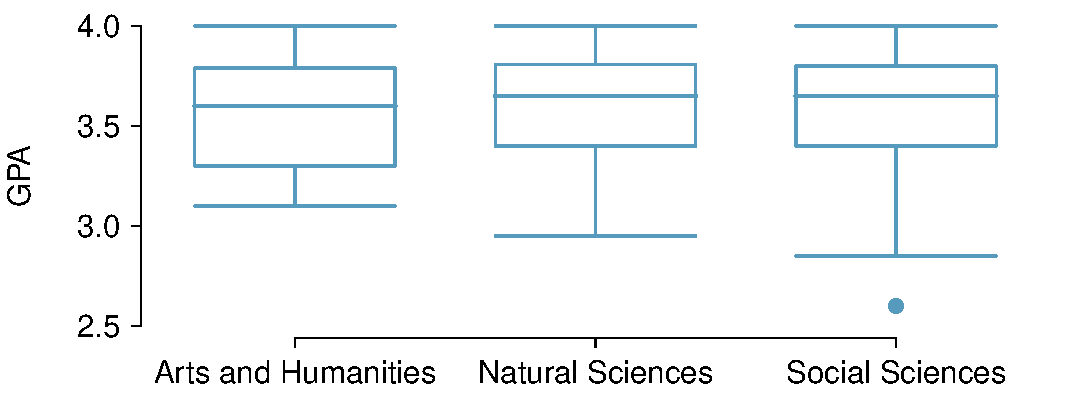
\includegraphics[width=0.85\textwidth]{ch_inference_for_means/figures/eoce/gpa_major/gpa_major.pdf}
\end{center}
\begin{center}
\begin{tabular}{lrrrrr}
  \hline
            & Df    & Sum Sq    & Mean Sq   & F value   & Pr($>$F) \\ 
  \hline
major       & 2     & 0.03      & 0.015      & 0.185     & 0.8313 \\ 
Residuals   & 195   & 15.77     & 0.081      &           &  \\ 
   \hline
\end{tabular}
\end{center}
\begin{parts}
\item Write the hypotheses for testing for a difference between average GPA across majors.
\item What is the conclusion of the hypothesis test?
\item How many students answered these questions on the survey, i.e. what is the sample size?
\end{parts}
}{}

% 8

\eoce{\qt{Work hours and education\label{work_hours_education}} The General Social Survey 
collects data on demographics, education, and work, among many other characteristics 
of US residents. \footfullcite{data:gss} Using ANOVA, we can consider 
educational attainment levels for all 1,172 respondents at once. Below are the 
distributions of hours worked by educational attainment and relevant summary 
statistics that will be helpful in carrying out this analysis.
\begin{center}

\begin{tabular}{l  r  r  r  r  r  r}
                & \multicolumn{5}{c}{\textit{Educational attainment}} \\
\cline{2-6}
                & Less than HS  & HS    & Jr Coll   & Bachelor's & Graduate & Total \\
\hline
Mean            & 38.67         & 39.6  & 41.39     & 42.55     & 40.85     & 40.45 \\
SD              & 15.81         & 14.97 & 18.1      & 13.62     & 15.51     & 15.17 \\
n               & 121           & 546   & 97        & 253       & 155       & 1,172 \\
\hline
\end{tabular}

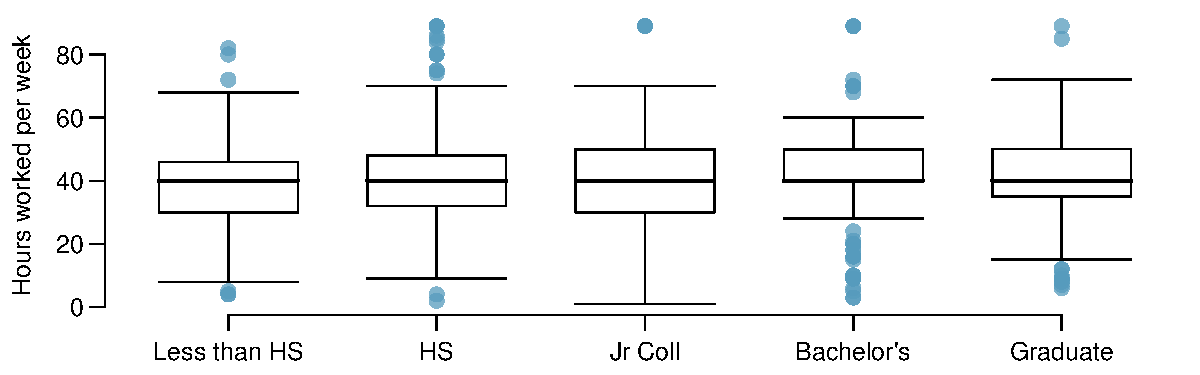
\includegraphics[width=\textwidth]{ch_inference_for_means/figures/eoce/work_hours_education/work_hours_education.pdf}
\end{center}
\begin{parts}
\item Write hypotheses for evaluating whether the average number of hours 
worked varies across the five groups.
\item Check conditions and describe any assumptions you must make to proceed 
with the test.
\item Below is part of the output associated with this test. Fill in the 
empty cells.

\begin{center}
\renewcommand{\arraystretch}{1.25}
\begin{tabular}{lrrrrr}
  \hline
            & Df    
                    & Sum Sq        
                            & Mean Sq       
                                    & F-value      
                                            & Pr($>$F) \\ 
  \hline
degree      & \fbox{\textcolor{white}{{\footnotesize XXXXX}}}       
                    & \fbox{\textcolor{white}{{\footnotesize XXXXX}}}       
                            & 501.54    
                                    & \fbox{\textcolor{white}{{\footnotesize XXXXX}}}   
                                            & 0.0682 \\ 
Residuals   & \fbox{\textcolor{white}{{\footnotesize XXXXX}}} 
                    & 267,382     
                            & \fbox{\textcolor{white}{{\footnotesize  XXXXX}}}          
                                    &       
                                            &  \\ 
   \hline
Total       & \fbox{\textcolor{white}{{\footnotesize XXXXX}}} 
                    &\fbox{\textcolor{white}{{\footnotesize XXXXX}}}
\end{tabular}
\end{center}

\item What is the conclusion of the test?

\end{parts}
}{}

% 9

\eoce{\qt{True / False: ANOVA, Part I\label{tf_anova_1}} Determine if the following statements are true or false in ANOVA, and explain your reasoning for statements you identify as false.
\begin{parts}
\item As the number of groups increases, the modified significance level for pairwise tests increases as well.
\item As the total sample size increases, the degrees of freedom for the residuals increases as well.
\item The constant variance condition can be somewhat relaxed when the sample sizes are relatively consistent across groups.
\item The independence assumption can be relaxed when the total sample size is large.
\end{parts}
}{}

% 10

\eoce{\qt{Child care hours\label{child_care_hours}} The China Health and Nutrition 
Survey aims to examine the effects of the health, nutrition, and family planning 
policies and programs implemented by national and local governments.\footfullcite{data:china} It, for example, collects information on number of hours Chinese parents spend 
taking care of their children under age 6. The side-by-side box plots below 
show the distribution of this variable by educational attainment of the parent. 
Also provided below is the ANOVA output for comparing average hours across 
educational attainment categories.
\begin{center}
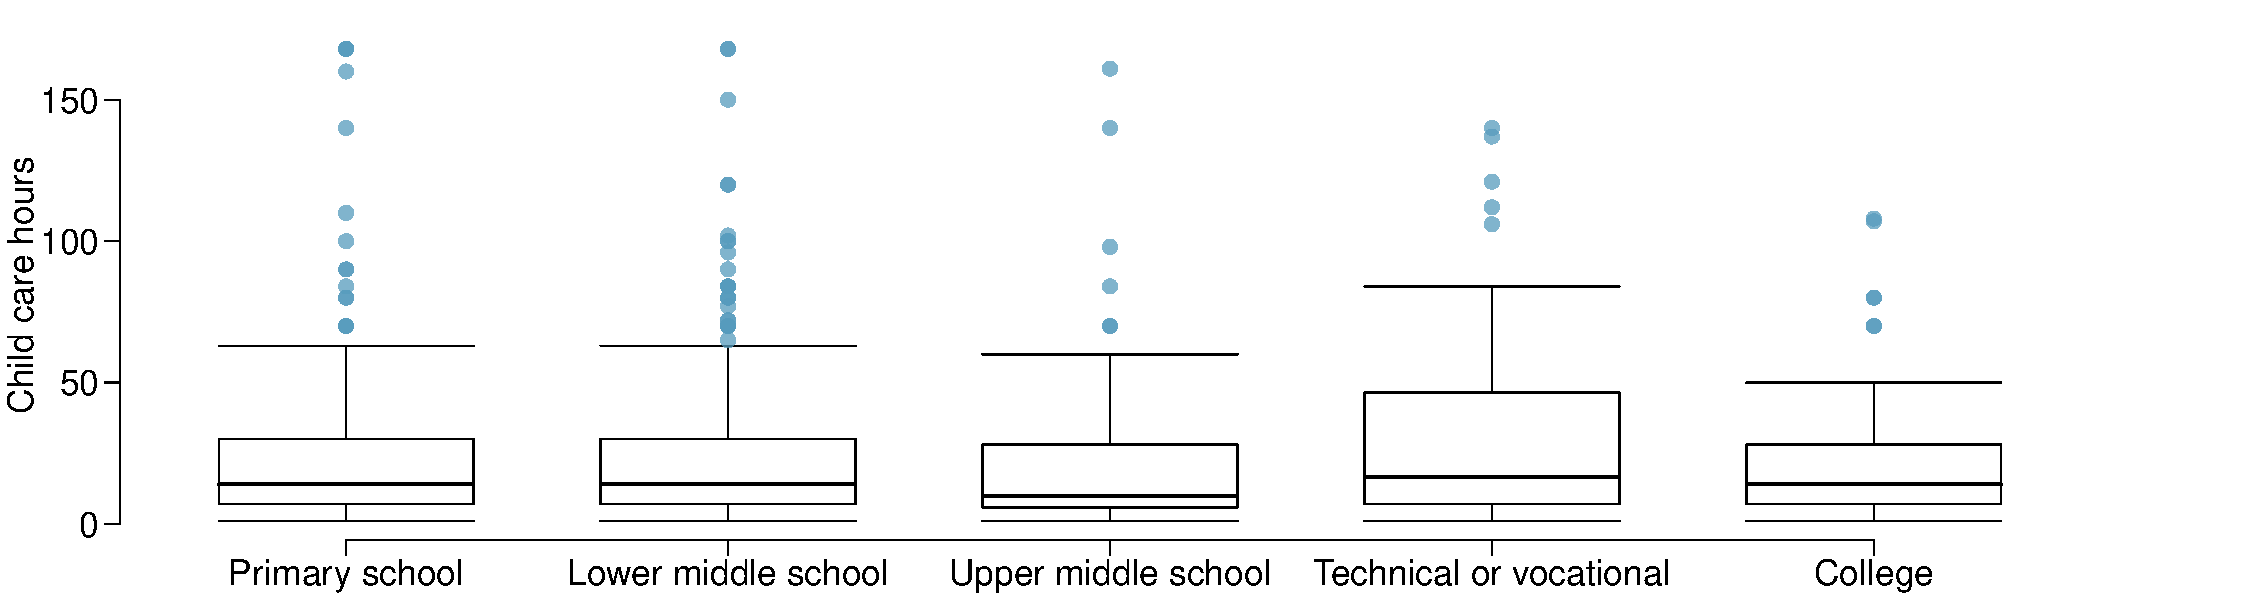
\includegraphics[width=\textwidth]{ch_inference_for_means/figures/eoce/child_care_hours/child_care_hours.pdf}
\end{center}
\begin{center}
\begin{tabular}{lrrrrr}
\hline
            & Df    & Sum Sq    & Mean Sq   & F value   & Pr($>$F) \\ 
\hline
education   & 4     & 4142.09   & 1035.52   & 1.26      & 0.2846 \\ 
Residuals   & 794   & 653047.83 & 822.48    &           &  \\ 
\hline
\end{tabular}
\end{center}
\begin{parts}
\item Write the hypotheses for testing for a difference between the average 
number of hours spent on child care across educational attainment levels.
\item What is the conclusion of the hypothesis test?
\end{parts}
}{}

% 11

\eoce{\qt{Prison isolation experiment, Part II\label{prison_isolation_anova}} Exercise~\ref{prison_isolation_T} introduced an experiment that was conducted with the goal of identifying a treatment that reduces subjects' psychopathic deviant T scores, where this score measures a person's need for control or his rebellion against control. In Exercise~\ref{prison_isolation_T} you evaluated the success of each treatment individually. An alternative analysis involves comparing the success of treatments. The relevant ANOVA output is given below.
\begin{center}
\begin{tabular}{lrrrrr}
  \hline
 & Df & Sum Sq & Mean Sq & F value & Pr($>$F) \\ 
  \hline
treatment & 2 & 639.48 & 319.74 & 3.33 & 0.0461 \\ 
  Residuals & 39 & 3740.43 & 95.91 &  &  \\ 
   \hline
\multicolumn{6}{r}{$s_{pooled} = 9.793$ on $df=39$}
\end{tabular}
\end{center}
\begin{parts}
\item What are the hypotheses?
\item What is the conclusion of the test? Use a 5\% significance level.
\item If in part~(b) you determined that the test is significant, conduct pairwise tests to determine which groups are different from each other. If you did not reject the null hypothesis in part~(b), recheck your answer.
\end{parts}
}{}

% 12

\eoce{\qt{True / False: ANOVA, Part II\label{tf_anova_2}} Determine if the following statements are true or false, and explain your reasoning for statements you identify as false.

If the null hypothesis that the means of four groups are all the same is rejected using ANOVA at a 5\% significance level, then ...
\begin{parts}
\item we can then conclude that all the means are different from one another.
\item the standardized variability between groups is higher than the standardized variability within groups.
\item the pairwise analysis will identify at least one pair of means that are significantly different.
\item the appropriate $\alpha$ to be used in pairwise comparisons is 0.05 / 4 = 0.0125 since there are four groups.
\end{parts}
}{}
}
